% ---------------------------------------------------------------- 25e Dual model: two trunks, one head
\begin{frame}{The dual model --- two trunks, one head}
  \begin{columns}[c]
    \begin{column}{0.54\textwidth}
      \centering
      \begin{tikzpicture}[font=\scriptsize, scale=0.92, transform shape,
          exc/.style={-{Stealth[length=1.8mm]}, argA!85, thick, densely dashed}]
        % parameter input card
        \begin{scope}[shift={(0,2.1)}]
          \draw[soft,thin,rounded corners=3pt,fill=black!2] (0,0) rectangle (2.05,1.42);
          \foreach \i in {3,2,1} \draw[soft,thin,fill=black!2] (0.26+0.05*\i,0.48+0.05*\i) rectangle ++(0.55,0.55);
          \draw[soft,thin,fill=white] (0.26,0.48) rectangle ++(0.55,0.55);
          \draw[black!8,xstep=0.1375,ystep=0.1375,shift={(0.26,0.48)}] (0,0) grid (0.55,0.55);
          \foreach \i in {3,2,1} \draw[soft,thin,fill=black!2] (1.16+0.05*\i,0.48+0.05*\i) rectangle ++(0.55,0.55);
          \draw[soft,thin,fill=white] (1.16,0.48) rectangle ++(0.55,0.55);
          \begin{scope} \clip (1.16,0.48) rectangle ++(0.55,0.55); \foreach \r in {0.25,0.37,...,1.2} \draw[accent!30,thin] (1.86,0.23) circle (\r); \end{scope}
          \node[font=\tiny,text=soft] at (0.61,0.26) {5 $|A|$};
          \node[font=\tiny,text=soft] at (1.49,0.26) {4 $\varphi$};
          \node[font=\tiny\bfseries,text=soft,anchor=south] at (1.025,1.45) {parameter input};
        \end{scope}
        % existence input card
        \begin{scope}[shift={(0,-1.0)}]
          \draw[soft,thin,rounded corners=3pt,fill=black!2] (0,0) rectangle (2.05,1.42);
          \foreach \i in {3,2,1} \draw[soft,thin,fill=black!2] (0.26+0.05*\i,0.48+0.05*\i) rectangle ++(0.55,0.55);
          \draw[soft,thin,fill=white] (0.26,0.48) rectangle ++(0.55,0.55);
          \draw[black!8,xstep=0.1375,ystep=0.1375,shift={(0.26,0.48)}] (0,0) grid (0.55,0.55);
          \foreach \i in {3,2,1} \draw[soft,thin,fill=black!2] (1.16+0.05*\i,0.48+0.05*\i) rectangle ++(0.55,0.55);
          \draw[soft,thin,fill=white] (1.16,0.48) rectangle ++(0.55,0.55);
          \begin{scope} \clip (1.16,0.48) rectangle ++(0.55,0.55); \foreach \r in {0.25,0.37,...,1.2} \draw[accent!30,thin] (1.86,0.23) circle (\r); \end{scope}
          \node[font=\tiny,text=soft] at (0.61,0.26) {5 $|A|$};
          \node[font=\tiny,text=soft] at (1.49,0.26) {4 $\varphi$};
          \node[font=\tiny\bfseries,text=soft,anchor=south] at (1.025,1.45) {existence input};
        \end{scope}
        % trunks, heads, outputs
        \node[box, minimum width=21mm, minimum height=12mm] (tp) at (3.5,2.81)  {parameter trunk\\(UNet-skip)};
        \node[box, minimum width=21mm, minimum height=12mm] (te) at (3.5,-0.29) {existence trunk\\(UNet-skip)};
        \node[gate, minimum height=9mm]  (gh) at (5.65,2.81)  {Gaussian\\heads $1..K$};
        \node[gate, minimum height=9mm]  (eh) at (5.65,-0.29) {existence\\head};
        \node[gate, draw=accent!70, fill=accent!8, minimum height=7mm] (op) at (7.5,2.81) {$\hat a_k,\mu_k,\sigma_k$};
        \node[font=\scriptsize, text=good] (gk) at (7.5,-0.29) {$g_k{=}\sigma(e_k)$};
        \draw[flow] (2.05,2.81) -- (tp.west);
        \draw[flow] (2.05,-0.29) -- (te.west);
        \draw[flow] (tp.east) -- (gh.west);
        \draw[flow] (te.east) -- (eh.west);
        \draw[flow] (gh.east) -- (op.west);
        \draw[flow] (eh.east) -- node[midway, above, font=\tiny]{$e_k$} (gk.west);
        \draw[exc] (gk.north) -- node[midway, right, font=\tiny, text=argA, align=left]{gates\\the blend} (op.south);
      \end{tikzpicture}
      \\[8pt]
      {\footnotesize each gate:\; $a_k = g_k\,\hat a_k + (1-g_k)\,a_{\mathrm{off},k}$}\\[1pt]
      {\scriptsize\color{soft} the set-prediction head of Act III, unchanged --- only the source of each embedding splits\par}
    \end{column}
    \begin{column}{0.43\textwidth}
      \small
      The gated head asks two questions per slot: \emph{is a scatterer there}
      ($g_k$) and \emph{what is it} ($\hat a_k,\mu_k,\sigma_k$). So far one
      backbone embedding had to answer both.
      \par\smallskip
      \begin{itemize}\setlength{\itemsep}{5pt}
        \item \textbf{Split the encoder, keep the head}: two independent UNet-skip
              trunks --- the Gaussian heads read one embedding, the existence
              head the other. Gate blend and Hungarian matching stay as they are.
        \item \textbf{Each trunk picks its own stack}: the channel groups $|A|$
              (5 amplitudes) and $\varphi$ (4 interferograms) are selected
              per trunk --- which modality reaches which head becomes an
              architectural choice.
        \item \textbf{Why route}: the input ablation split the labour --- phase
              fires the slots, the full stack calibrates the parameters. The
              dual model can hand each head the input its job needs.
        \item[\textcolor{accent}{$\blacksquare$}] \textbf{Default routing}: the
              full stack $\to$ parameter trunk, $\varphi$ alone $\to$ existence
              trunk.
      \end{itemize}
    \end{column}
  \end{columns}
\end{frame}

% ---------------------------------------------------------------- 25f Dual routing experiment
\begin{frame}{Routing the trunks --- which stack in front of which head?}
  \begin{columns}[c]
    \begin{column}{0.50\textwidth}
      \centering
      \begin{tikzpicture}[font=\scriptsize, scale=0.92, transform shape,
          pics/ampg/.style={code={\draw[soft,thin,fill=white] (0,0) rectangle (0.42,0.42);\draw[black!8,xstep=0.105,ystep=0.105] (0,0) grid (0.42,0.42);}},
          pics/phg/.style={code={\begin{scope}\clip (0,0) rectangle (0.42,0.42);\foreach \r in {0.19,0.29,...,0.95} \draw[accent!30,thin] (0.52,-0.1) circle (\r);\end{scope}\draw[soft,thin] (0,0) rectangle (0.42,0.42);}}]
        % headers
        \node[font=\scriptsize\bfseries,text=soft] at (3.075,6.0) {existence trunk (gate) input};
        \node[font=\scriptsize,text=soft] at (1.025,5.55) {$|A|{+}\varphi$};
        \node[font=\scriptsize,text=soft] at (3.375,5.55) {$\varphi$};
        \node[font=\scriptsize,text=soft] at (5.725,5.55) {$|A|$};
        \node[font=\scriptsize\bfseries,text=soft,rotate=90] at (-1.05,2.5) {parameter trunk input};
        \node[font=\scriptsize,text=soft,rotate=90] at (-0.5,4.25) {$|A|{+}\varphi$};
        \node[font=\scriptsize,text=soft,rotate=90] at (-0.5,2.5)  {$\varphi$};
        \node[font=\scriptsize,text=soft,rotate=90] at (-0.5,0.75) {$|A|$};
        % row 1: params = both
        \begin{scope}[shift={(0,3.5)}]
          \draw[soft!80,thick,rounded corners=3pt,fill=black!2] (0,0) rectangle (2.05,1.5);
          \node[font=\tiny,text=soft,anchor=north east] at (2.0,1.47) {reference};
          \node[font=\tiny,text=soft] at (0.26,1.01) {par};
          \pic at (0.52,0.80) {ampg}; \pic at (1.12,0.80) {phg};
          \draw[soft!35,thin] (0.1,0.68) -- (1.95,0.68);
          \node[font=\tiny,text=soft] at (0.26,0.33) {gate};
          \pic at (0.52,0.12) {ampg}; \pic at (1.12,0.12) {phg};
        \end{scope}
        \begin{scope}[shift={(2.35,3.5)}]
          \draw[accent!70,thick,rounded corners=3pt,fill=accent!4] (0,0) rectangle (2.05,1.5);
          \node[font=\tiny,text=accent,anchor=north east] at (2.0,1.47) {default};
          \node[font=\tiny,text=soft] at (0.26,1.01) {par};
          \pic at (0.52,0.80) {ampg}; \pic at (1.12,0.80) {phg};
          \draw[soft!35,thin] (0.1,0.68) -- (1.95,0.68);
          \node[font=\tiny,text=soft] at (0.26,0.33) {gate};
          \pic at (0.82,0.12) {phg};
        \end{scope}
        \begin{scope}[shift={(4.7,3.5)}]
          \draw[soft,thin,rounded corners=3pt,fill=black!2] (0,0) rectangle (2.05,1.5);
          \node[font=\tiny,text=soft] at (0.26,1.01) {par};
          \pic at (0.52,0.80) {ampg}; \pic at (1.12,0.80) {phg};
          \draw[soft!35,thin] (0.1,0.68) -- (1.95,0.68);
          \node[font=\tiny,text=soft] at (0.26,0.33) {gate};
          \pic at (0.82,0.12) {ampg};
        \end{scope}
        % row 2: params = phase
        \begin{scope}[shift={(0,1.75)}]
          \draw[soft,thin,rounded corners=3pt,fill=black!2] (0,0) rectangle (2.05,1.5);
          \node[font=\tiny,text=soft] at (0.26,1.01) {par};
          \pic at (0.82,0.80) {phg};
          \draw[soft!35,thin] (0.1,0.68) -- (1.95,0.68);
          \node[font=\tiny,text=soft] at (0.26,0.33) {gate};
          \pic at (0.52,0.12) {ampg}; \pic at (1.12,0.12) {phg};
        \end{scope}
        \begin{scope}[shift={(2.35,1.75)}]
          \draw[soft!60,thin,dashed,rounded corners=3pt] (0,0) rectangle (2.05,1.5);
          \node[font=\tiny,text=soft] at (1.025,0.75) {not run};
        \end{scope}
        \begin{scope}[shift={(4.7,1.75)}]
          \draw[soft,thin,rounded corners=3pt,fill=black!2] (0,0) rectangle (2.05,1.5);
          \node[font=\tiny,text=soft] at (0.26,1.01) {par};
          \pic at (0.82,0.80) {phg};
          \draw[soft!35,thin] (0.1,0.68) -- (1.95,0.68);
          \node[font=\tiny,text=soft] at (0.26,0.33) {gate};
          \pic at (0.82,0.12) {ampg};
        \end{scope}
        % row 3: params = amplitude
        \begin{scope}[shift={(0,0)}]
          \draw[soft,thin,rounded corners=3pt,fill=black!2] (0,0) rectangle (2.05,1.5);
          \node[font=\tiny,text=soft] at (0.26,1.01) {par};
          \pic at (0.82,0.80) {ampg};
          \draw[soft!35,thin] (0.1,0.68) -- (1.95,0.68);
          \node[font=\tiny,text=soft] at (0.26,0.33) {gate};
          \pic at (0.52,0.12) {ampg}; \pic at (1.12,0.12) {phg};
        \end{scope}
        \begin{scope}[shift={(2.35,0)}]
          \draw[soft,thin,rounded corners=3pt,fill=black!2] (0,0) rectangle (2.05,1.5);
          \node[font=\tiny,text=soft] at (0.26,1.01) {par};
          \pic at (0.82,0.80) {ampg};
          \draw[soft!35,thin] (0.1,0.68) -- (1.95,0.68);
          \node[font=\tiny,text=soft] at (0.26,0.33) {gate};
          \pic at (0.82,0.12) {phg};
        \end{scope}
        \begin{scope}[shift={(4.7,0)}]
          \draw[soft!60,thin,dashed,rounded corners=3pt] (0,0) rectangle (2.05,1.5);
          \node[font=\tiny,text=soft] at (1.025,0.75) {not run};
        \end{scope}
      \end{tikzpicture}
      \\[5pt]
      {\scriptsize\color{soft} 7 routings $\times$ 5 seeds $=$ 35 runs\par}
    \end{column}
    \begin{column}{0.46\textwidth}
      \small
      The trunks stay identical twins --- every arm holds
      ${\approx}31.2$\,M parameters --- so the arms differ only in what each
      trunk sees.
      \par\smallskip
      \begin{itemize}\setlength{\itemsep}{5pt}
        \item \textbf{The grid}: parameter-trunk input $\times$ gate input over
              $\{|A|{+}\varphi,\ \varphi,\ |A|\}$; the two single-modality
              diagonal cells are omitted.
        \item \textbf{H1 --- the parameter trunk needs phase}: with $|A|$ alone
              in front of the parameters the curve should collapse, and no gate
              input can buy it back.
        \item \textbf{H2 --- the gate runs on phase alone}: the default routing
              should match the all-channels reference everywhere.
        \item \textbf{H3 --- the reversed default pays on the curve}:
              $\varphi\to$ parameters should keep detection but give up
              reconstruction, mirroring the ablation's phase-only arm.
      \end{itemize}
    \end{column}
  \end{columns}
\end{frame}

% ---------------------------------------------------------------- 25g Dual routing: the verdict
\begin{frame}{The verdict --- the parameter trunk sets the tier, the gate input is nearly free}
    \centering
  \scriptsize
  \renewcommand{\arraystretch}{0.98}
  \setlength{\tabcolsep}{4pt}
  \renewcommand{\seedtag}{dlA}
  \begin{tabular}{@{}l ccc !{\hspace{9pt}} cc !{\hspace{9pt}} cc@{}}
    \toprule
    & \multicolumn{3}{c}{params $|A|{+}\varphi$} & \multicolumn{2}{c}{params $\varphi$} & \multicolumn{2}{c@{}}{params $|A|$} \\
    \cmidrule(lr){2-4}\cmidrule(lr){5-6}\cmidrule(l){7-8}
    metric & $|A|{+}\varphi$ & $\varphi$ & $|A|$ & $|A|{+}\varphi$ & $|A|$ & $|A|{+}\varphi$ & $\varphi$ \\
    \midrule
    \multicolumn{8}{@{}l}{\emph{training (validation)}} \\
    val loss $\downarrow$ & \seedpm{0.189}{.001} & \seedpm{\textbf{0.188}}{.001} & \seedpm{0.189}{.001} & \seedpm{0.196}{.001} & \seedpm{0.197}{.001} & \seedpm{0.222}{.002} & \seedpm{0.224}{.001} \\
    \addlinespace
    \multicolumn{8}{@{}l}{\emph{reconstruction (curve)}} \\
    curve $R^2$ $\uparrow$ & \seedpm{0.738}{.006} & \seedpm{0.730}{.009} & \seedpm{\textbf{0.741}}{.007} & \seedpm{0.690}{.010} & \seedpm{0.685}{.009} & \seedpm{\hlval{accent}{0.489}}{.013} & \seedpm{\hlval{accent}{0.493}}{.017} \\
    curve MAE $\downarrow$ & \seedpm{\textbf{0.037}}{.000} & \seedpm{0.038}{.001} & \seedpm{\textbf{0.037}}{.000} & \seedpm{0.039}{.000} & \seedpm{0.040}{.000} & \seedpm{0.054}{.000} & \seedpm{0.055}{.001} \\
    PSNR [dB] $\uparrow$ & \seedpm{\textbf{52.5}}{.1} & \seedpm{52.3}{.1} & \seedpm{\textbf{52.5}}{.1} & \seedpm{51.8}{.1} & \seedpm{51.7}{.1} & \seedpm{49.6}{.1} & \seedpm{49.6}{.1} \\
    SSIM elev $\uparrow$ & \seedpm{0.967}{.000} & \seedpm{0.967}{.000} & \seedpm{0.967}{.000} & \seedpm{0.966}{.000} & \seedpm{0.965}{.000} & \seedpm{0.956}{.000} & \seedpm{0.955}{.001} \\
    SSIM range $\uparrow$ & \seedpm{0.951}{.000} & \seedpm{0.951}{.001} & \seedpm{0.951}{.000} & \seedpm{0.949}{.000} & \seedpm{0.948}{.001} & \seedpm{0.927}{.001} & \seedpm{0.926}{.001} \\
    SSIM azim $\uparrow$ & \seedpm{0.961}{.000} & \seedpm{0.960}{.001} & \seedpm{0.961}{.000} & \seedpm{0.959}{.000} & \seedpm{0.958}{.000} & \seedpm{0.943}{.000} & \seedpm{0.942}{.001} \\
    profile cos med\,$\uparrow$ & \seedpm{\textbf{0.967}}{.002} & \seedpm{0.966}{.007} & \seedpm{\textbf{0.967}}{.002} & \seedpm{0.961}{.007} & \seedpm{0.963}{.004} & \seedpm{0.887}{.009} & \seedpm{0.881}{.007} \\
    \addlinespace
    \multicolumn{8}{@{}l}{\emph{detection (matched)}} \\
    precision $\uparrow$ & \seedpm{0.905}{.001} & \seedpm{\textbf{0.907}}{.002} & \seedpm{0.901}{.003} & \seedpm{0.892}{.006} & \seedpm{0.892}{.011} & \seedpm{0.836}{.015} & \seedpm{0.843}{.014} \\
    recall $\uparrow$ & \seedpm{0.892}{.002} & \seedpm{0.884}{.004} & \seedpm{0.890}{.004} & \seedpm{0.893}{.005} & \seedpm{0.886}{.004} & \seedpm{0.862}{.004} & \seedpm{0.852}{.003} \\
    matched F1 $\uparrow$ & \seedpm{\textbf{0.898}}{.001} & \seedpm{0.895}{.003} & \seedpm{0.896}{.003} & \seedpm{0.893}{.003} & \seedpm{0.889}{.004} & \seedpm{0.849}{.008} & \seedpm{0.848}{.006} \\
    count exact $\uparrow$ & \seedpm{\textbf{0.914}}{.001} & \seedpm{0.907}{.003} & \seedpm{0.909}{.006} & \seedpm{0.908}{.003} & \seedpm{0.904}{.002} & \seedpm{0.870}{.023} & \seedpm{0.864}{.014} \\
    peak err med $\downarrow$ & \seedpm{0.27}{.37} & \seedpm{\textbf{0.13}}{.30} & \seedpm{0.40}{.37} & \seedpm{0.40}{.37} & \seedpm{0.54}{.30} & \seedpm{0.67}{.00} & \seedpm{0.67}{.00} \\
    peak err p95 $\downarrow$ & \seedpm{5.4}{.0} & \seedpm{6.0}{.5} & \seedpm{5.5}{.3} & \seedpm{\textbf{5.0}}{.4} & \seedpm{5.8}{.6} & \seedpm{7.5}{.6} & \seedpm{8.1}{.0} \\
    \bottomrule
    \end{tabular}
  \par\vspace{3pt}
  \parbox{0.82\textwidth}{\tiny\color{soft} \textbf{runs}: dual UNet-skip trunks $\cdot$ set-pred $\cdot$ Hungarian $\cdot$ $K{=}2$ $\cdot$ param-L1 $\cdot$ presence A $\cdot$ full norm ladder $\cdot$ hv flips $\cdot$ patch $64{\times}32$ $\cdot$ symmetric twin trunks, ${\approx}31.2$\,M params per arm. Column group $=$ parameter-trunk input, sub-column $=$ existence (gate) trunk input; $|A|{+}\varphi$ $=$ 5 amplitudes $+$ 4 interferograms. Five seeded replicas per arm, cells mean $\pm$ seed std; held-out test, $5.0$\,M px. \textbf{bold} $=$ best in row, marked only where best and worst differ by more than $5\%$; \textcolor{accent}{red} $=$ the curve price of an amplitude-only parameter trunk; matched $=$ Hungarian pairing. Peak err med/p95: per-pixel peak-error distribution; profile cos med: median per-pixel cosine to the GT profile.\par}
    

\end{frame}

% ---------------------------------------------------------------- 25h Dual routing by scatterer count
\begin{frame}{Dual routing by scatterer count --- detection survives without phase, position does not}
    \centering
  \scriptsize
  \renewcommand{\arraystretch}{1.02}
  \setlength{\tabcolsep}{4pt}
  \renewcommand{\seedtag}{dlB}
  \begin{tabular}{@{}l ccc !{\hspace{9pt}} cc !{\hspace{9pt}} cc@{}}
    \toprule
    & \multicolumn{3}{c}{params $|A|{+}\varphi$} & \multicolumn{2}{c}{params $\varphi$} & \multicolumn{2}{c@{}}{params $|A|$} \\
    \cmidrule(lr){2-4}\cmidrule(lr){5-6}\cmidrule(l){7-8}
    metric & $|A|{+}\varphi$ & $\varphi$ & $|A|$ & $|A|{+}\varphi$ & $|A|$ & $|A|{+}\varphi$ & $\varphi$ \\
    \midrule
    precision $\uparrow$ & \seedpm{0.905}{.001} & \seedpm{\textbf{0.907}}{.002} & \seedpm{0.901}{.003} & \seedpm{0.892}{.006} & \seedpm{0.892}{.011} & \seedpm{0.836}{.015} & \seedpm{0.843}{.014} \\
    \quad $k{=}1$ & \seedpm{0.949}{.002} & \seedpm{\textbf{0.952}}{.002} & \seedpm{0.944}{.005} & \seedpm{0.938}{.007} & \seedpm{0.940}{.009} & \seedpm{0.889}{.025} & \seedpm{0.898}{.021} \\
    \quad $k{=}2$ & \seedpm{\textbf{0.831}}{.001} & \seedpm{\textbf{0.831}}{.004} & \seedpm{0.829}{.002} & \seedpm{0.816}{.005} & \seedpm{0.812}{.014} & \seedpm{0.745}{.006} & \seedpm{0.749}{.006} \\
    \addlinespace
    recall $\uparrow$ & \seedpm{0.892}{.002} & \seedpm{0.884}{.004} & \seedpm{0.890}{.004} & \seedpm{0.893}{.005} & \seedpm{0.886}{.004} & \seedpm{0.862}{.004} & \seedpm{0.852}{.003} \\
    \quad $k{=}1$ & \seedpm{0.997}{.001} & \seedpm{0.992}{.002} & \seedpm{0.996}{.002} & \seedpm{0.998}{.000} & \seedpm{0.998}{.001} & \seedpm{0.991}{.002} & \seedpm{0.980}{.007} \\
    \quad $k{=}2$ & \seedpm{\textbf{0.743}}{.004} & \seedpm{0.729}{.006} & \seedpm{0.740}{.008} & \seedpm{\textbf{0.743}}{.011} & \seedpm{0.727}{.010} & \seedpm{0.680}{.007} & \seedpm{0.670}{.008} \\
    \addlinespace
    \multicolumn{8}{@{}l}{\emph{count acc $\mid$ pred $k$}} \\
    \quad pred $k{=}1$ $\uparrow$ & \seedpm{0.953}{.003} & \seedpm{0.947}{.003} & \seedpm{0.953}{.002} & \seedpm{0.941}{.008} & \seedpm{0.939}{.005} & \seedpm{0.958}{.009} & \seedpm{0.946}{.002} \\
    \quad pred $k{=}2$ $\uparrow$ & \seedpm{0.846}{.003} & \seedpm{\textbf{0.851}}{.005} & \seedpm{0.834}{.012} & \seedpm{0.820}{.015} & \seedpm{0.822}{.017} & \seedpm{0.718}{.051} & \seedpm{0.732}{.045} \\
    \addlinespace
    $\mu$ MAE $\downarrow$ & \seedpm{1.63}{.01} & \seedpm{\hlval{good}{\textbf{1.59}}}{.04} & \seedpm{1.63}{.02} & \seedpm{1.73}{.06} & \seedpm{1.74}{.16} & \seedpm{2.35}{.07} & \seedpm{2.31}{.03} \\
    \quad $k{=}1$ & \seedpm{\textbf{0.33}}{.01} & \seedpm{\textbf{0.33}}{.03} & \seedpm{\textbf{0.33}}{.02} & \seedpm{0.37}{.03} & \seedpm{0.36}{.03} & \seedpm{\hlval{accent}{0.79}}{.06} & \seedpm{\hlval{accent}{0.79}}{.03} \\
    \quad $k{=}2$ & \seedpm{3.70}{.02} & \seedpm{\textbf{3.62}}{.06} & \seedpm{3.70}{.04} & \seedpm{3.85}{.08} & \seedpm{3.93}{.31} & \seedpm{4.77}{.16} & \seedpm{4.68}{.05} \\
    \addlinespace
    $\sigma$ MAE $\downarrow$ & \seedpm{0.694}{.005} & \seedpm{0.692}{.006} & \seedpm{\hlval{good}{\textbf{0.691}}}{.007} & \seedpm{0.783}{.032} & \seedpm{0.763}{.050} & \seedpm{0.828}{.037} & \seedpm{0.851}{.007} \\
    \quad $k{=}1$ & \seedpm{\textbf{0.185}}{.002} & \seedpm{0.189}{.006} & \seedpm{\textbf{0.185}}{.003} & \seedpm{0.221}{.013} & \seedpm{0.210}{.013} & \seedpm{0.235}{.013} & \seedpm{0.246}{.009} \\
    \quad $k{=}2$ & \seedpm{1.503}{.009} & \seedpm{1.503}{.014} & \seedpm{\textbf{1.495}}{.018} & \seedpm{1.660}{.056} & \seedpm{1.640}{.090} & \seedpm{1.746}{.072} & \seedpm{1.798}{.011} \\
    \addlinespace
    $a$ MAE $\downarrow$ & \seedpm{\textbf{0.181}}{.003} & \seedpm{0.182}{.002} & \seedpm{0.184}{.002} & \seedpm{0.185}{.004} & \seedpm{0.191}{.007} & \seedpm{0.192}{.015} & \seedpm{0.191}{.004} \\
    \quad $k{=}1$ & \seedpm{\textbf{0.056}}{.001} & \seedpm{\textbf{0.056}}{.002} & \seedpm{0.059}{.001} & \seedpm{0.061}{.003} & \seedpm{0.063}{.003} & \seedpm{0.066}{.009} & \seedpm{0.066}{.004} \\
    \quad $k{=}2$ & \seedpm{0.380}{.006} & \seedpm{0.385}{.005} & \seedpm{0.382}{.003} & \seedpm{0.380}{.009} & \seedpm{0.395}{.019} & \seedpm{0.387}{.023} & \seedpm{0.387}{.006} \\
    \bottomrule
    \end{tabular}
  \par\vspace{3pt}
  \parbox{0.82\textwidth}{\tiny\color{soft} \textbf{runs}: dual UNet-skip trunks $\cdot$ set-pred $\cdot$ Hungarian $\cdot$ $K{=}2$ $\cdot$ param-L1 $\cdot$ presence A $\cdot$ full norm ladder $\cdot$ hv flips $\cdot$ patch $64{\times}32$ $\cdot$ symmetric twin trunks. Column group $=$ parameter-trunk input, sub-column $=$ gate-trunk input. All precision / recall / $\mu$ / $\sigma$ / $a$ rows are matched (Hungarian pairing). Cells mean $\pm$ seed std over five seeded replicas; held-out test; $k$ $=$ true scatterer count of the pixel. \textbf{bold} $=$ best in row, marked only where best and worst differ by more than $5\%$; \textcolor{good}{green} $=$ the sharpest localisation, both on a full-parameter trunk, \textcolor{accent}{red} $=$ position dying without phase. Precision rewards under-prediction --- rank on recall. count acc $\mid$ pred $k$: share of pixels claiming exactly $k$ scatterers whose true count is $k$. $\mu$, $\sigma$ in elevation units; $a$ in linear amplitude.\par}
    

\end{frame}

% ---------------------------------------------------------------- 25i Dual routing: predicted stats vs GT
\begin{frame}{Dual routing, predicted statistics vs the GT --- calibration follows the parameter trunk}
    \centering
  \scriptsize
  \renewcommand{\arraystretch}{0.90}
  \setlength{\tabcolsep}{2.5pt}
  \renewcommand{\seedtag}{dlC}
  \begin{tabular}{@{}l !{\color{white}\vrule width 0.6pt} c !{\color{white}\vrule width 0.6pt} ccc !{\hspace{7pt}} cc !{\hspace{7pt}} cc@{}}
    \toprule
    & & \multicolumn{3}{c}{params $|A|{+}\varphi$} & \multicolumn{2}{c}{params $\varphi$} & \multicolumn{2}{c@{}}{params $|A|$} \\
    \cmidrule(lr){3-5}\cmidrule(lr){6-7}\cmidrule(l){8-9}
    mean & \textcolor{good}{GT} & $|A|{+}\varphi$ & $\varphi$ & $|A|$ & $|A|{+}\varphi$ & $|A|$ & $|A|{+}\varphi$ & $\varphi$ \\
    \midrule
    \multicolumn{9}{@{}l}{\textcolor{soft}{\emph{slot 0 --- strongest scatterer; GT-active on every pixel}}} \\
    \; active frac & 1.000 & \seedpm{0.973}{.002} & \seedpm{0.968}{.002} & \seedpm{0.973}{.003} & \seedpm{\hlval{good}{0.983}}{.005} & \seedpm{0.977}{.006} & \seedpm{0.978}{.007} & \seedpm{0.969}{.006} \\
    \; $a$ --- active & 0.77 & \seedpm{0.72}{.01} & \seedpm{\textbf{0.76}}{.01} & \seedpm{0.72}{.01} & \seedpm{0.72}{.02} & \seedpm{0.72}{.01} & \seedpm{0.73}{.01} & \seedpm{0.73}{.01} \\
    \; $\mu$ --- active & $-4.89$ & \seedpm{$-4.57$}{.04} & \seedpm{$-4.53$}{.04} & \seedpm{$-4.54$}{.05} & \seedpm{$-4.56$}{.04} & \seedpm{$-4.52$}{.07} & \seedpm{$-4.46$}{.10} & \seedpm{$-4.49$}{.08} \\
    \; $\sigma$ --- active & 1.76 & \seedpm{1.35}{.02} & \seedpm{1.34}{.01} & \seedpm{1.37}{.02} & \seedpm{1.39}{.03} & \seedpm{1.36}{.03} & \seedpm{1.38}{.03} & \seedpm{1.37}{.03} \\
    \addlinespace[1.5pt]
    \multicolumn{9}{@{}l}{\textcolor{soft}{\emph{slot 1 --- second scatterer; GT-active on 26\% of pixels}}} \\
    \; active frac & 0.260 & \seedpm{0.269}{.003} & \seedpm{\hlval{good}{\textbf{0.260}}}{.002} & \seedpm{0.272}{.004} & \seedpm{0.278}{.009} & \seedpm{0.274}{.015} & \seedpm{0.322}{.025} & \seedpm{0.305}{.021} \\
    \; $a$ --- active & 1.43 & \seedpm{1.43}{.01} & \seedpm{1.47}{.03} & \seedpm{1.42}{.03} & \seedpm{1.44}{.06} & \seedpm{1.38}{.05} & \seedpm{1.39}{.07} & \seedpm{1.44}{.02} \\
    \; $a$ --- inact. & 0.00 & \seedpm{0.87}{.04} & \seedpm{0.90}{.06} & \seedpm{0.82}{.09} & \seedpm{0.78}{.05} & \seedpm{0.75}{.15} & \seedpm{\textbf{0.53}}{.10} & \seedpm{0.57}{.10} \\
    \; $\mu$ --- active & 11.34 & \seedpm{7.66}{.13} & \seedpm{7.70}{.24} & \seedpm{7.72}{.26} & \seedpm{7.68}{.37} & \seedpm{\textbf{8.15}}{.38} & \seedpm{6.96}{.31} & \seedpm{7.04}{.26} \\
    \; $\mu$ --- inact. & --- & \seedpm{0.82}{.16} & \seedpm{0.94}{.38} & \seedpm{0.50}{.48} & \seedpm{0.67}{.57} & \seedpm{0.44}{.93} & \seedpm{$-0.35$}{1.18} & \seedpm{$-0.86$}{.87} \\
    \; $\sigma$ --- active & 3.53 & \seedpm{3.23}{.06} & \seedpm{3.21}{.06} & \seedpm{3.24}{.02} & \seedpm{\textbf{3.29}}{.10} & \seedpm{3.28}{.06} & \seedpm{3.14}{.06} & \seedpm{3.10}{.05} \\
    \; $\sigma$ --- inact. & --- & \seedpm{1.81}{.02} & \seedpm{1.79}{.04} & \seedpm{1.79}{.09} & \seedpm{1.89}{.02} & \seedpm{1.83}{.07} & \seedpm{2.00}{.26} & \seedpm{1.85}{.26} \\
    \addlinespace[1.5pt]
    \multicolumn{9}{@{}l}{\textcolor{soft}{\emph{distribution width --- std over GT-active pixels}}} \\
    \; $a$ --- slot 0 & 1.48 & \seedpm{1.28}{.03} & \seedpm{\textbf{1.35}}{.02} & \seedpm{1.25}{.03} & \seedpm{1.20}{.04} & \seedpm{1.18}{.03} & \seedpm{1.30}{.03} & \seedpm{1.33}{.04} \\
    \; $\mu$ --- slot 0 & 3.30 & \seedpm{2.33}{.07} & \seedpm{2.22}{.09} & \seedpm{2.35}{.07} & \seedpm{2.32}{.09} & \seedpm{\textbf{2.46}}{.21} & \seedpm{2.38}{.29} & \seedpm{2.35}{.41} \\
    \; $\sigma$ --- slot 0 & 2.84 & \seedpm{1.15}{.04} & \seedpm{1.15}{.04} & \seedpm{1.16}{.04} & \seedpm{\textbf{1.23}}{.09} & \seedpm{1.15}{.06} & \seedpm{1.12}{.08} & \seedpm{1.14}{.14} \\
    \; $a$ --- slot 1 & 1.45 & \seedpm{1.28}{.02} & \seedpm{\textbf{1.29}}{.02} & \seedpm{1.26}{.05} & \seedpm{1.26}{.07} & \seedpm{1.20}{.03} & \seedpm{1.24}{.05} & \seedpm{1.28}{.01} \\
    \; $\mu$ --- slot 1 & 16.24 & \seedpm{8.85}{.09} & \seedpm{8.62}{.37} & \seedpm{8.78}{.34} & \seedpm{8.63}{.38} & \seedpm{\textbf{9.56}}{.75} & \seedpm{7.81}{.28} & \seedpm{7.71}{.14} \\
    \; $\sigma$ --- slot 1 & 4.01 & \seedpm{\textbf{1.72}}{.03} & \seedpm{1.69}{.04} & \seedpm{1.67}{.05} & \seedpm{1.58}{.08} & \seedpm{1.59}{.04} & \seedpm{1.32}{.04} & \seedpm{1.26}{.05} \\
    \bottomrule
    \end{tabular}
  \par\vspace{3pt}
  \parbox{0.82\textwidth}{\tiny\color{soft} \textbf{runs}: dual UNet-skip trunks $\cdot$ set-pred $\cdot$ Hungarian $\cdot$ $K{=}2$ $\cdot$ param-L1 $\cdot$ presence A $\cdot$ full norm ladder $\cdot$ hv flips $\cdot$ patch $64{\times}32$ $\cdot$ symmetric twin trunks. Column group $=$ parameter-trunk input, sub-column $=$ gate-trunk input. Five seeded replicas per arm, cells mean $\pm$ seed std; means conditioned on the slot's GT activity mask. \textbf{bold} $=$ closest to the \textcolor{good}{GT} column, marked only where best and worst differ by more than $5\%$; \textcolor{good}{green} $=$ calibration following the parameter trunk; inactive GT slots define no $\mu$/$\sigma$ reference (---). Width rows: std of the prediction over GT-active pixels vs the GT's own std. $\mu$, $\sigma$ in elevation units; $a$ in linear amplitude.\par}
    

\end{frame}

% ---------------------------------------------------------------- 25j Dual routing at K=5: headline
\begin{frame}{Dual routing at $K{=}5$ --- the parameter trunk still sets the tier, the gate turns conservative}
    \centering
  \scriptsize
  \renewcommand{\arraystretch}{0.95}
  \setlength{\tabcolsep}{4pt}
  \renewcommand{\seedtag}{kdA}
  \begin{tabular}{@{}l ccc !{\hspace{9pt}} cc !{\hspace{9pt}} cc@{}}
    \toprule
    & \multicolumn{3}{c}{params $|A|{+}\varphi$} & \multicolumn{2}{c}{params $\varphi$} & \multicolumn{2}{c@{}}{params $|A|$} \\
    \cmidrule(lr){2-4}\cmidrule(lr){5-6}\cmidrule(l){7-8}
    metric & $|A|{+}\varphi$ & $\varphi$ & $|A|$ & $|A|{+}\varphi$ & $|A|$ & $|A|{+}\varphi$ & $\varphi$ \\
    \midrule
    \multicolumn{8}{@{}l}{\emph{training (validation)}} \\
    val loss $\downarrow$ & \seedpm{0.130}{.000} & \seedpm{\textbf{0.129}}{.000} & \seedpm{\textbf{0.129}}{.000} & \seedpm{0.133}{.000} & \seedpm{0.135}{.001} & \seedpm{0.143}{.001} & \seedpm{0.148}{.002} \\
    \addlinespace
    \multicolumn{8}{@{}l}{\emph{reconstruction (curve)}} \\
    curve $R^2$ $\uparrow$ & \seedpm{0.679}{.010} & \seedpm{0.676}{.005} & \seedpm{\textbf{0.680}}{.014} & \seedpm{0.624}{.007} & \seedpm{0.635}{.015} & \seedpm{\hlval{accent}{0.458}}{.011} & \seedpm{\hlval{accent}{0.475}}{.014} \\
    curve MAE $\downarrow$ & \seedpm{0.046}{.000} & \seedpm{0.046}{.001} & \seedpm{\textbf{0.045}}{.000} & \seedpm{0.047}{.000} & \seedpm{0.047}{.001} & \seedpm{0.062}{.001} & \seedpm{0.062}{.002} \\
    PSNR [dB] $\uparrow$ & \seedpm{51.0}{.1} & \seedpm{51.0}{.1} & \seedpm{51.0}{.2} & \seedpm{50.3}{.1} & \seedpm{50.5}{.2} & \seedpm{48.7}{.1} & \seedpm{48.9}{.1} \\
    SSIM elev $\uparrow$ & \seedpm{0.961}{.000} & \seedpm{0.961}{.000} & \seedpm{0.962}{.000} & \seedpm{0.961}{.000} & \seedpm{0.960}{.001} & \seedpm{0.953}{.000} & \seedpm{0.953}{.001} \\
    SSIM range $\uparrow$ & \seedpm{0.940}{.001} & \seedpm{0.940}{.001} & \seedpm{0.940}{.001} & \seedpm{0.939}{.001} & \seedpm{0.938}{.003} & \seedpm{0.921}{.003} & \seedpm{0.920}{.004} \\
    SSIM azim $\uparrow$ & \seedpm{0.954}{.000} & \seedpm{0.954}{.000} & \seedpm{0.955}{.000} & \seedpm{0.953}{.000} & \seedpm{0.953}{.001} & \seedpm{0.939}{.001} & \seedpm{0.940}{.002} \\
    profile cos med\,$\uparrow$ & \seedpm{0.922}{.011} & \seedpm{\textbf{0.932}}{.005} & \seedpm{0.927}{.005} & \seedpm{0.920}{.008} & \seedpm{0.922}{.015} & \seedpm{0.795}{.041} & \seedpm{0.791}{.065} \\
    \addlinespace
    \multicolumn{8}{@{}l}{\emph{detection (matched)}} \\
    precision $\uparrow$ & \seedpm{0.917}{.006} & \seedpm{0.917}{.003} & \seedpm{0.915}{.004} & \seedpm{0.916}{.010} & \seedpm{0.900}{.011} & \seedpm{0.891}{.012} & \seedpm{0.875}{.026} \\
    recall $\uparrow$ & \seedpm{0.666}{.008} & \seedpm{0.671}{.018} & \seedpm{0.670}{.026} & \seedpm{0.697}{.025} & \seedpm{0.673}{.066} & \seedpm{0.661}{.081} & \seedpm{\textbf{0.706}}{.050} \\
    matched F1 $\uparrow$ & \seedpm{0.772}{.007} & \seedpm{0.774}{.011} & \seedpm{0.774}{.017} & \seedpm{0.791}{.016} & \seedpm{0.769}{.046} & \seedpm{0.757}{.056} & \seedpm{0.780}{.026} \\
    count exact $\uparrow$ & \seedpm{0.632}{.012} & \seedpm{0.638}{.022} & \seedpm{0.635}{.035} & \seedpm{0.669}{.030} & \seedpm{0.628}{.085} & \seedpm{0.648}{.103} & \seedpm{\textbf{0.675}}{.048} \\
    \quad under $\downarrow$ & \seedpm{0.329}{.011} & \seedpm{0.323}{.023} & \seedpm{0.325}{.037} & \seedpm{0.289}{.031} & \seedpm{0.323}{.084} & \seedpm{0.310}{.109} & \seedpm{\textbf{0.251}}{.070} \\
    \quad over $\downarrow$ & \seedpm{\textbf{0.039}}{.003} & \seedpm{\textbf{0.039}}{.003} & \seedpm{0.040}{.002} & \seedpm{0.041}{.008} & \seedpm{0.049}{.004} & \seedpm{0.043}{.011} & \seedpm{0.074}{.040} \\
    peak err med $\downarrow$ & \seedpm{\textbf{0.67}}{.00} & \seedpm{\textbf{0.67}}{.00} & \seedpm{\textbf{0.67}}{.00} & \seedpm{\textbf{0.67}}{.00} & \seedpm{\textbf{0.67}}{.00} & \seedpm{\hlval{accent}{1.07}}{.37} & \seedpm{\hlval{accent}{1.07}}{.37} \\
    peak err p95 $\downarrow$ & \seedpm{14.1}{.0} & \seedpm{14.1}{.0} & \seedpm{14.1}{.0} & \seedpm{13.7}{.6} & \seedpm{\textbf{13.2}}{2.1} & \seedpm{\textbf{13.2}}{1.5} & \seedpm{13.6}{1.1} \\
    \bottomrule
    \end{tabular}
  \par\vspace{3pt}
  \parbox{0.82\textwidth}{\tiny\color{soft} \textbf{runs}: dual UNet-skip trunks $\cdot$ set-pred $\cdot$ Hungarian $\cdot$ $K{=}5$ $\cdot$ param-L1 $\cdot$ presence A $\cdot$ full norm ladder $\cdot$ hv flips $\cdot$ patch $64{\times}32$ $\cdot$ symmetric parity-twin trunks, ${\approx}31.2$\,M params per arm. Column group $=$ parameter-trunk input, sub-column $=$ existence (gate) trunk input; $|A|{+}\varphi$ $=$ 5 amplitudes $+$ 4 interferograms. Five seeded replicas per arm, cells mean $\pm$ seed std; held-out test, $5.0$\,M px, $K_{\max}{=}5$ labels. \textbf{bold} $=$ best in row, marked only where best and worst differ by more than $5\%$; \textcolor{accent}{red} $=$ the curve price of an amplitude-only parameter trunk. under / over $=$ predicted count below / above the GT count: the dual misses tail scatterers (under 0.25--0.33, over ${\leq}0.07$) --- the opposite failure of the $K{=}5$ single-trunk arms. Peak err med/p95: per-pixel peak-error distribution; profile cos med: median per-pixel cosine to the GT profile.\par}
\end{frame}

% ---------------------------------------------------------------- 25k Dual routing at K=5 by scatterer count
\begin{frame}{The $K{=}5$ dual by scatterer count --- $k{=}1$ no longer saturates, recall fades up the ladder}
    \centering
  \scriptsize
  \renewcommand{\arraystretch}{1.0}
  \setlength{\tabcolsep}{4pt}
  \renewcommand{\seedtag}{kdB}
  \begin{tabular}{@{}l ccc !{\hspace{9pt}} cc !{\hspace{9pt}} cc@{}}
    \toprule
    & \multicolumn{3}{c}{params $|A|{+}\varphi$} & \multicolumn{2}{c}{params $\varphi$} & \multicolumn{2}{c@{}}{params $|A|$} \\
    \cmidrule(lr){2-4}\cmidrule(lr){5-6}\cmidrule(l){7-8}
    metric & $|A|{+}\varphi$ & $\varphi$ & $|A|$ & $|A|{+}\varphi$ & $|A|$ & $|A|{+}\varphi$ & $\varphi$ \\
    \midrule
    precision $\uparrow$ & \seedpm{0.917}{.006} & \seedpm{0.917}{.003} & \seedpm{0.915}{.004} & \seedpm{0.916}{.010} & \seedpm{0.900}{.011} & \seedpm{0.891}{.012} & \seedpm{0.875}{.026} \\
    \quad $k{=}1$ & \seedpm{\textbf{0.936}}{.005} & \seedpm{0.935}{.004} & \seedpm{0.935}{.004} & \seedpm{0.934}{.013} & \seedpm{0.908}{.015} & \seedpm{0.921}{.013} & \seedpm{0.890}{.038} \\
    \quad $k{=}2$ & \seedpm{0.912}{.008} & \seedpm{0.911}{.004} & \seedpm{\textbf{0.913}}{.009} & \seedpm{0.910}{.004} & \seedpm{0.910}{.007} & \seedpm{0.848}{.007} & \seedpm{0.856}{.009} \\
    \quad $k{=}3$ & \seedpm{0.869}{.010} & \seedpm{0.871}{.010} & \seedpm{0.864}{.016} & \seedpm{0.869}{.006} & \seedpm{0.872}{.013} & \seedpm{0.842}{.005} & \seedpm{0.848}{.009} \\
    \quad $k{=}4$ & \seedpm{0.819}{.013} & \seedpm{0.820}{.019} & \seedpm{0.805}{.028} & \seedpm{0.815}{.014} & \seedpm{0.820}{.018} & \seedpm{0.809}{.009} & \seedpm{0.812}{.013} \\
    \quad $k{=}5$ & \seedpm{0.794}{.015} & \seedpm{0.791}{.028} & \seedpm{0.769}{.042} & \seedpm{0.780}{.022} & \seedpm{0.783}{.020} & \seedpm{0.787}{.017} & \seedpm{0.790}{.016} \\
    \addlinespace
    recall $\uparrow$ & \seedpm{0.666}{.008} & \seedpm{0.671}{.018} & \seedpm{0.670}{.026} & \seedpm{0.697}{.025} & \seedpm{0.673}{.066} & \seedpm{0.661}{.081} & \seedpm{\textbf{0.706}}{.050} \\
    \quad $k{=}1$ & \seedpm{0.757}{.014} & \seedpm{0.766}{.031} & \seedpm{0.761}{.047} & \seedpm{0.807}{.038} & \seedpm{0.768}{\hlval{accent}{.109}} & \seedpm{0.787}{\hlval{accent}{.143}} & \seedpm{\textbf{0.858}}{\hlval{accent}{.093}} \\
    \quad $k{=}2$ & \seedpm{0.701}{.008} & \seedpm{0.700}{.007} & \seedpm{\textbf{0.708}}{.006} & \seedpm{0.707}{.025} & \seedpm{0.704}{.023} & \seedpm{\hlval{accent}{0.632}}{.011} & \seedpm{\hlval{accent}{0.657}}{.011} \\
    \quad $k{=}3$ & \seedpm{0.508}{.005} & \seedpm{0.507}{.006} & \seedpm{0.509}{.004} & \seedpm{\textbf{0.510}}{.010} & \seedpm{0.506}{.008} & \seedpm{0.472}{.003} & \seedpm{0.477}{.009} \\
    \quad $k{=}4$ & \seedpm{0.358}{.008} & \seedpm{0.356}{.005} & \seedpm{0.360}{.004} & \seedpm{\textbf{0.362}}{.009} & \seedpm{0.359}{.010} & \seedpm{0.331}{.006} & \seedpm{0.332}{.007} \\
    \quad $k{=}5$ & \seedpm{0.239}{.008} & \seedpm{0.239}{.005} & \seedpm{0.242}{.006} & \seedpm{\textbf{0.257}}{.011} & \seedpm{0.251}{.016} & \seedpm{0.219}{.008} & \seedpm{0.219}{.008} \\
    \addlinespace
    \multicolumn{8}{@{}l}{\emph{count acc $\mid$ pred $k$ $\uparrow$}} \\
    \quad pred $k{=}1$ & \seedpm{0.885}{.005} & \seedpm{0.887}{.005} & \seedpm{0.887}{.006} & \seedpm{0.888}{.012} & \seedpm{0.868}{.020} & \seedpm{0.873}{.018} & \seedpm{0.884}{.006} \\
    \quad pred $k{=}2$ & \seedpm{\textbf{0.496}}{.005} & \seedpm{0.488}{.006} & \seedpm{0.493}{.003} & \seedpm{0.485}{.007} & \seedpm{0.469}{.011} & \seedpm{0.454}{.023} & \seedpm{0.413}{.063} \\
    \quad pred $k{=}3$ & \seedpm{\textbf{0.252}}{.012} & \seedpm{0.236}{.015} & \seedpm{0.243}{.008} & \seedpm{0.239}{.009} & \seedpm{0.164}{.054} & \seedpm{0.207}{.024} & \seedpm{0.147}{.067} \\
    \quad pred $k{=}4$ & \seedpm{0.198}{.014} & \seedpm{0.188}{.016} & \seedpm{\textbf{0.210}}{.013} & \seedpm{0.198}{.020} & \seedpm{0.110}{.066} & \seedpm{0.180}{.052} & \seedpm{0.169}{.027} \\
    \quad pred $k{=}5$ & \seedpm{0.198}{.039} & \seedpm{0.196}{.071} & \seedpm{0.222}{.024} & \seedpm{0.183}{.045} & \seedpm{0.142}{.072} & \seedpm{0.129}{.067} & \seedpm{\textbf{0.306}}{.393} \\
    \bottomrule
    \end{tabular}
  \par\vspace{3pt}
  \parbox{0.82\textwidth}{\tiny\color{soft} \textbf{runs}: dual UNet-skip trunks $\cdot$ set-pred $\cdot$ Hungarian $\cdot$ $K{=}5$ $\cdot$ param-L1 $\cdot$ presence A $\cdot$ full norm ladder $\cdot$ hv flips $\cdot$ patch $64{\times}32$ $\cdot$ symmetric parity-twin trunks. Column group $=$ parameter-trunk input, sub-column $=$ gate-trunk input. All precision / recall rows are matched (Hungarian pairing). Cells mean $\pm$ seed std over five seeded replicas; held-out test; $k$ $=$ true scatterer count of the pixel. \textbf{bold} $=$ best in row, marked only where best and worst differ by more than $5\%$; \textcolor{accent}{red} $=$ the two-scatterer price of a phase-free parameter trunk, and the $k{=}1$ seed lottery (coloured $\pm$ spreads). Precision rewards under-prediction --- rank on recall. count acc $\mid$ pred $k$: share of pixels claiming exactly $k$ scatterers whose true count is $k$.\par}
\end{frame}

% ---------------------------------------------------------------- 25l Dual routing at K=5: component errors
\begin{frame}{The $K{=}5$ dual components --- position pays for the crowd, and doubly without phase}
    \centering
  \scriptsize
  \renewcommand{\arraystretch}{1.0}
  \setlength{\tabcolsep}{4pt}
  \renewcommand{\seedtag}{kdC}
  \begin{tabular}{@{}l ccc !{\hspace{9pt}} cc !{\hspace{9pt}} cc@{}}
    \toprule
    & \multicolumn{3}{c}{params $|A|{+}\varphi$} & \multicolumn{2}{c}{params $\varphi$} & \multicolumn{2}{c@{}}{params $|A|$} \\
    \cmidrule(lr){2-4}\cmidrule(lr){5-6}\cmidrule(l){7-8}
    metric & $|A|{+}\varphi$ & $\varphi$ & $|A|$ & $|A|{+}\varphi$ & $|A|$ & $|A|{+}\varphi$ & $\varphi$ \\
    \midrule
    $\mu$ MAE $\downarrow$ & \seedpm{1.16}{.05} & \seedpm{\textbf{1.15}}{.03} & \seedpm{1.17}{.03} & \seedpm{1.19}{.05} & \seedpm{1.18}{.08} & \seedpm{1.73}{.12} & \seedpm{1.74}{.18} \\
    \quad $k{=}1$ & \seedpm{0.48}{.03} & \seedpm{\textbf{0.45}}{.01} & \seedpm{0.46}{.02} & \seedpm{0.51}{.02} & \seedpm{0.49}{.02} & \seedpm{\hlval{accent}{1.02}}{.09} & \seedpm{\hlval{accent}{1.13}}{.23} \\
    \quad $k{=}2$ & \seedpm{\textbf{1.81}}{.03} & \seedpm{1.88}{.05} & \seedpm{1.83}{.06} & \seedpm{1.90}{.03} & \seedpm{1.91}{.08} & \seedpm{\hlval{accent}{2.76}}{.06} & \seedpm{\hlval{accent}{2.69}}{.06} \\
    \quad $k{=}3$ & \seedpm{2.55}{.18} & \seedpm{2.48}{.14} & \seedpm{2.51}{.09} & \seedpm{2.54}{.12} & \seedpm{\textbf{2.43}}{.13} & \seedpm{2.92}{.04} & \seedpm{2.90}{.15} \\
    \quad $k{=}4$ & \seedpm{3.26}{.26} & \seedpm{3.20}{.27} & \seedpm{3.34}{.32} & \seedpm{3.26}{.24} & \seedpm{\textbf{3.05}}{.21} & \seedpm{3.30}{.10} & \seedpm{3.30}{.25} \\
    \quad $k{=}5$ & \seedpm{3.52}{.23} & \seedpm{3.48}{.45} & \seedpm{3.83}{.54} & \seedpm{3.55}{.31} & \seedpm{3.49}{.36} & \seedpm{3.45}{.20} & \seedpm{\textbf{3.43}}{.26} \\
    \addlinespace
    $\sigma$ MAE $\downarrow$ & \seedpm{\textbf{0.60}}{.01} & \seedpm{\textbf{0.60}}{.01} & \seedpm{\textbf{0.60}}{.02} & \seedpm{0.63}{.02} & \seedpm{0.64}{.03} & \seedpm{0.70}{.07} & \seedpm{0.67}{.04} \\
    \quad $k{=}1$ & \seedpm{\textbf{0.27}}{.01} & \seedpm{\textbf{0.27}}{.00} & \seedpm{\textbf{0.27}}{.01} & \seedpm{0.28}{.01} & \seedpm{0.29}{.02} & \seedpm{0.33}{.03} & \seedpm{0.32}{.03} \\
    \quad $k{=}2$ & \seedpm{\textbf{0.88}}{.01} & \seedpm{0.89}{.01} & \seedpm{0.89}{.01} & \seedpm{0.94}{.01} & \seedpm{0.95}{.02} & \seedpm{1.14}{.02} & \seedpm{1.11}{.02} \\
    \quad $k{=}3$ & \seedpm{\textbf{1.31}}{.02} & \seedpm{1.33}{.01} & \seedpm{1.33}{.02} & \seedpm{1.37}{.02} & \seedpm{1.36}{.02} & \seedpm{1.50}{.02} & \seedpm{1.47}{.02} \\
    \quad $k{=}4$ & \seedpm{\textbf{1.65}}{.02} & \seedpm{1.66}{.02} & \seedpm{1.68}{.03} & \seedpm{1.76}{.03} & \seedpm{1.75}{.04} & \seedpm{1.75}{.02} & \seedpm{1.74}{.04} \\
    \quad $k{=}5$ & \seedpm{\textbf{1.83}}{.02} & \seedpm{1.84}{.03} & \seedpm{1.85}{.03} & \seedpm{2.02}{.05} & \seedpm{2.02}{.09} & \seedpm{1.90}{.04} & \seedpm{1.91}{.10} \\
    \addlinespace
    $a$ MAE $\downarrow$ & \seedpm{0.212}{.005} & \seedpm{\textbf{0.198}}{.002} & \seedpm{0.205}{.011} & \seedpm{0.199}{.007} & \seedpm{0.225}{.023} & \seedpm{\textbf{0.198}}{.014} & \seedpm{0.201}{.017} \\
    \quad $k{=}1$ & \seedpm{0.076}{.004} & \seedpm{\textbf{0.073}}{.003} & \seedpm{0.077}{.008} & \seedpm{0.079}{.005} & \seedpm{0.094}{.012} & \seedpm{0.077}{.009} & \seedpm{0.076}{.011} \\
    \quad $k{=}2$ & \seedpm{0.387}{.013} & \seedpm{\textbf{0.366}}{.013} & \seedpm{0.371}{.015} & \seedpm{0.370}{.008} & \seedpm{0.400}{.017} & \seedpm{0.375}{.017} & \seedpm{0.399}{.032} \\
    \quad $k{=}3$ & \seedpm{0.464}{.013} & \seedpm{\textbf{0.431}}{.008} & \seedpm{0.440}{.012} & \seedpm{0.436}{.007} & \seedpm{0.465}{.027} & \seedpm{0.433}{.014} & \seedpm{0.466}{.029} \\
    \quad $k{=}4$ & \seedpm{0.498}{.016} & \seedpm{0.448}{.008} & \seedpm{0.466}{.015} & \seedpm{\textbf{0.440}}{.013} & \seedpm{0.477}{.039} & \seedpm{0.442}{.018} & \seedpm{0.475}{.029} \\
    \quad $k{=}5$ & \seedpm{0.498}{.023} & \seedpm{0.440}{.018} & \seedpm{0.456}{.017} & \seedpm{\textbf{0.403}}{.017} & \seedpm{0.455}{.059} & \seedpm{0.414}{.023} & \seedpm{0.446}{.035} \\
    \bottomrule
    \end{tabular}
  \par\vspace{3pt}
  \parbox{0.82\textwidth}{\tiny\color{soft} \textbf{runs}: dual UNet-skip trunks $\cdot$ set-pred $\cdot$ Hungarian $\cdot$ $K{=}5$ $\cdot$ param-L1 $\cdot$ presence A $\cdot$ full norm ladder $\cdot$ hv flips $\cdot$ patch $64{\times}32$ $\cdot$ symmetric parity-twin trunks. Column group $=$ parameter-trunk input, sub-column $=$ gate-trunk input. Cells mean $\pm$ seed std over five seeded replicas; held-out test; $k$ $=$ true scatterer count of the pixel; component errors over matched pairs only --- low-recall arms are graded on an easier subset. \textbf{bold} $=$ best in row, marked only where best and worst differ by more than $5\%$; \textcolor{accent}{red} $=$ position paying double without phase in the parameter trunk. $\mu$, $\sigma$ in elevation units; $a$ in linear amplitude.\par}
\end{frame}

% ---------------------------------------------------------------- 25m Dual routing at K=5: predicted stats vs GT
\begin{frame}{The $K{=}5$ dual, predicted statistics vs the GT --- the always-active slot fires on three quarters of the pixels}
    \centering
  \scriptsize
  \renewcommand{\arraystretch}{0.82}
  \setlength{\tabcolsep}{2.5pt}
  \renewcommand{\seedtag}{kdD}
  \begin{tabular}{@{}l !{\color{white}\vrule width 0.6pt} c !{\color{white}\vrule width 0.6pt} ccc !{\hspace{7pt}} cc !{\hspace{7pt}} cc@{}}
    \toprule
    & & \multicolumn{3}{c}{params $|A|{+}\varphi$} & \multicolumn{2}{c}{params $\varphi$} & \multicolumn{2}{c@{}}{params $|A|$} \\
    \cmidrule(lr){3-5}\cmidrule(lr){6-7}\cmidrule(l){8-9}
    mean & \textcolor{good}{GT} & $|A|{+}\varphi$ & $\varphi$ & $|A|$ & $|A|{+}\varphi$ & $|A|$ & $|A|{+}\varphi$ & $\varphi$ \\
    \midrule
    \multicolumn{9}{@{}l}{\textcolor{soft}{\emph{predicted active fraction --- share of pixels where the slot fires}}} \\
    \; slot 0 & 1.000 & \seedpm{0.762}{.011} & \seedpm{0.768}{.020} & \seedpm{0.763}{.036} & \seedpm{0.802}{.029} & \seedpm{0.769}{.086} & \seedpm{0.790}{.107} & \seedpm{\textbf{0.847}}{.068} \\
    \; slot 1 & 0.239 & \seedpm{0.160}{.005} & \seedpm{0.161}{.003} & \seedpm{\textbf{0.169}}{.016} & \seedpm{\textbf{0.169}}{.013} & \seedpm{\textbf{0.169}}{.002} & \seedpm{0.168}{.014} & \seedpm{0.165}{.010} \\
    \; slot 2 & 0.085 & \seedpm{0.037}{.006} & \seedpm{\textbf{0.046}}{.007} & \seedpm{0.044}{.011} & \seedpm{\textbf{0.046}}{.017} & \seedpm{0.038}{.006} & \seedpm{0.038}{.012} & \seedpm{0.036}{.015} \\
    \; slot 3 & 0.035 & \seedpm{0.009}{.002} & \seedpm{0.008}{.002} & \seedpm{0.016}{.010} & \seedpm{0.013}{.009} & \seedpm{\textbf{0.036}}{.017} & \seedpm{0.013}{.012} & \seedpm{0.023}{.017} \\
    \; slot 4 & 0.015 & \seedpm{0.030}{.009} & \seedpm{0.022}{.013} & \seedpm{\textbf{0.014}}{.010} & \seedpm{0.016}{.019} & \seedpm{0.016}{.013} & \seedpm{0.008}{.008} & \seedpm{0.040}{.050} \\
    \addlinespace[1.5pt]
    \multicolumn{9}{@{}l}{\textcolor{soft}{\emph{$a$ --- predicted mean over GT-active pixels}}} \\
    \; slot 0 & 0.84 & \seedpm{0.94}{.02} & \seedpm{0.98}{.04} & \seedpm{0.95}{.04} & \seedpm{0.90}{.04} & \seedpm{0.91}{.09} & \seedpm{0.93}{.13} & \seedpm{\textbf{0.86}}{.06} \\
    \; slot 1 & 1.67 & \seedpm{1.82}{.04} & \seedpm{1.84}{.04} & \seedpm{1.82}{.06} & \seedpm{1.81}{.08} & \seedpm{1.76}{.11} & \seedpm{1.78}{.04} & \seedpm{\textbf{1.75}}{.03} \\
    \; slot 2 & 1.41 & \seedpm{1.81}{.03} & \seedpm{1.86}{.05} & \seedpm{\textbf{1.78}}{.11} & \seedpm{1.81}{.09} & \seedpm{1.80}{.09} & \seedpm{1.91}{.06} & \seedpm{1.86}{.09} \\
    \; slot 3 & 0.97 & \seedpm{1.29}{.06} & \seedpm{1.29}{.14} & \seedpm{1.15}{.17} & \seedpm{\textbf{1.13}}{.05} & \seedpm{1.32}{.07} & \seedpm{1.75}{.24} & \seedpm{1.58}{.11} \\
    \; slot 4 & 0.66 & \seedpm{\textbf{0.65}}{.10} & \seedpm{0.51}{.07} & \seedpm{0.55}{.06} & \seedpm{0.24}{.03} & \seedpm{0.57}{.09} & \seedpm{1.09}{.57} & \seedpm{0.61}{.31} \\
    \addlinespace[1.5pt]
    \multicolumn{9}{@{}l}{\textcolor{soft}{\emph{$a$ --- predicted mean over GT-inactive pixels (leakage)}}} \\
    \; slot 1 & 0.00 & \seedpm{0.79}{.86} & \seedpm{\textbf{0.50}}{.86} & \seedpm{0.92}{.67} & \seedpm{0.70}{.85} & \seedpm{0.59}{.67} & \seedpm{1.27}{.57} & \seedpm{0.59}{.75} \\
    \; slot 2 & 0.00 & \seedpm{0.69}{.60} & \seedpm{1.31}{.71} & \seedpm{0.98}{.72} & \seedpm{0.75}{.86} & \seedpm{0.50}{.67} & \seedpm{0.99}{.83} & \seedpm{\textbf{0.09}}{.03} \\
    \; slot 3 & 0.00 & \seedpm{0.33}{.19} & \seedpm{\textbf{0.26}}{.07} & \seedpm{0.82}{.64} & \seedpm{0.49}{.82} & \seedpm{0.92}{.53} & \seedpm{0.42}{.77} & \seedpm{0.84}{.68} \\
    \; slot 4 & 0.00 & \seedpm{1.53}{.16} & \seedpm{1.26}{.63} & \seedpm{0.91}{.84} & \seedpm{0.62}{.76} & \seedpm{0.68}{.73} & \seedpm{\textbf{0.41}}{.70} & \seedpm{0.76}{.83} \\
    \addlinespace[1.5pt]
    \multicolumn{9}{@{}l}{\textcolor{soft}{\emph{distribution width --- std over GT-active pixels}}} \\
    \; $a$ --- slot 0 & 1.59 & \seedpm{1.48}{.01} & \seedpm{\textbf{1.60}}{.04} & \seedpm{1.53}{.06} & \seedpm{1.41}{.04} & \seedpm{1.38}{.05} & \seedpm{1.50}{.11} & \seedpm{1.45}{.03} \\
    \; $\mu$ --- slot 0 & 3.02 & \seedpm{2.41}{.06} & \seedpm{2.44}{.08} & \seedpm{\textbf{2.51}}{.10} & \seedpm{2.41}{.09} & \seedpm{\textbf{2.51}}{.05} & \seedpm{2.35}{.08} & \seedpm{2.22}{.16} \\
    \; $\sigma$ --- slot 0 & 1.72 & \seedpm{1.03}{.04} & \seedpm{1.03}{.06} & \seedpm{1.04}{.06} & \seedpm{1.04}{.06} & \seedpm{\textbf{1.06}}{.09} & \seedpm{0.97}{.08} & \seedpm{0.91}{.06} \\
    \; $a$ --- slot 1 & 1.60 & \seedpm{1.38}{.03} & \seedpm{\textbf{1.43}}{.04} & \seedpm{1.41}{.03} & \seedpm{1.34}{.05} & \seedpm{1.37}{.05} & \seedpm{1.37}{.03} & \seedpm{1.34}{.06} \\
    \; $\mu$ --- slot 1 & 11.09 & \seedpm{\textbf{8.96}}{.40} & \seedpm{8.73}{.21} & \seedpm{8.77}{.22} & \seedpm{8.78}{.16} & \seedpm{8.74}{.29} & \seedpm{8.21}{.05} & \seedpm{7.75}{.42} \\
    \; $\sigma$ --- slot 1 & 2.30 & \seedpm{1.40}{.02} & \seedpm{1.40}{.04} & \seedpm{\textbf{1.43}}{.03} & \seedpm{1.32}{.03} & \seedpm{1.33}{.03} & \seedpm{1.31}{.07} & \seedpm{1.29}{.03} \\
    \bottomrule
    \end{tabular}
  \par\vspace{0pt}
  \parbox{0.82\textwidth}{\tiny\color{soft} \textbf{runs}: dual UNet-skip trunks $\cdot$ set-pred $\cdot$ Hungarian $\cdot$ $K{=}5$ $\cdot$ param-L1 $\cdot$ presence A $\cdot$ full norm ladder $\cdot$ hv flips $\cdot$ patch $64{\times}32$ $\cdot$ symmetric parity-twin trunks. Column group $=$ parameter-trunk input, sub-column $=$ gate-trunk input. Five seeded replicas per arm, cells mean $\pm$ seed std; means conditioned on the slot's GT activity mask. \textbf{bold} $=$ closest to the \textcolor{good}{GT} column, marked only where best and worst differ by more than $5\%$. The always-active slot 0 fires on 0.76--0.85 of pixels and slots 2--3 sit below their GT activity --- the $K{=}5$ dual gate under-counts rather than over-fires. Width rows: std of the prediction over GT-active pixels vs the GT's own std, shown for slots 0--1 (tail slots in the report). $\mu$, $\sigma$ in elevation units; $a$ in linear amplitude.\par}
\end{frame}

% ---------------------------------------------------------------- 25n Dual ratio experiment: the question
\begin{frame}{Splitting the budget --- how much of the model does detection need?}
  \begin{columns}[c]
    \begin{column}{0.53\textwidth}
      \centering
      \begin{tikzpicture}[font=\scriptsize, scale=0.84]
        \node[font=\tiny\bfseries,text=argA,anchor=south west] at (0,4.66) {parameter arm};
        \node[font=\tiny\bfseries,text=good,anchor=south east] at (6.0,4.66) {existence arm};
        \draw[decorate,decoration={brace,amplitude=4pt},soft] (0,5.12) -- (6.0,5.12);
        \node[font=\tiny,text=soft,anchor=south] at (3.0,5.28) {one budget: ${\approx}31.19$\,M parameters, totals within $0.1\%$};
        \foreach \y/\p/\lab/\pma/\ema in {4.0/3.0/50--50/15.6/15.6, 3.05/3.6/60--40/18.7/12.5, 2.1/4.2/70--30/21.8/9.4, 1.15/4.8/80--20/24.9/6.2, 0.2/5.4/90--10/28.1/3.1}{
          \draw[argA!70,thin,fill=argA!12] (0,\y) rectangle (\p,\y+0.52);
          \draw[good!70,thin,fill=good!12] (\p,\y) rectangle (6.0,\y+0.52);
          \node[font=\tiny,text=argA] at (\p/2,\y+0.26) {\pma\,M};
          \node[font=\tiny,text=good,anchor=west] at (6.08,\y+0.26) {\ema\,M};
          \node[font=\scriptsize,text=soft,anchor=east] at (-0.12,\y+0.26) {\lab};
        }
        \draw[soft,densely dashed] (3.0,-0.22) -- (3.0,4.62);
        \node[font=\tiny,text=soft,anchor=north] at (3.0,-0.26) {parity --- every dual run so far};
      \end{tikzpicture}
      \\[7pt]
      {\scriptsize\color{soft} 5 splits $\times$ 5 seeds, at $K{=}2$ and $K{=}5$ $=$ 50 runs; width scales like $\sqrt{\text{share}}$: the 10\% ladder (24--48--84--156) is half the parity width\par}
    \end{column}
    \begin{column}{0.43\textwidth}
      \footnotesize
      The routing block fixed \emph{what} each trunk sees. This experiment
      fixes the inputs and asks how one budget should be divided between the
      two arms.
      \par\smallskip
      \begin{itemize}\setlength{\itemsep}{3pt}
        \item \textbf{One budget, five splits}: the parity total is
              redistributed at fixed routing (the full stack in front of both
              trunks); ladders keep four levels, only width moves, and every
              realized split sits within $0.01$ points of its label.
        \item \textbf{An arm is trunk $+$ its heads}: every parameter belongs
              to exactly one arm; the 50--50 anchor is the routing block's
              all-channels reference arm.
        \item \textbf{H1 --- detection is cheap}: count and calibration hold
              to 80/20 or 90/10 and the freed capacity buys $\mu$/$\sigma$
              --- a better operating point than parity.
        \item \textbf{H2 --- parity is load-bearing}: count collapses as the
              existence arm shrinks, and the twins stand.
        \item \textbf{H3 --- the telling order}: $\mu$/$\sigma$ degrade before
              count does --- the gate was borrowing parameter-trunk capacity
              through the shared loss.
      \end{itemize}
    \end{column}
  \end{columns}
\end{frame}

% ---------------------------------------------------------------- 25o Dual ratio: the verdict
\begin{frame}{The ratio verdict --- detection survives on a tenth of the budget}
    \centering
  \scriptsize
  \renewcommand{\arraystretch}{0.98}
  \setlength{\tabcolsep}{6pt}
  \renewcommand{\seedtag}{drA}
  \begin{tabular}{@{}l ccccc !{\hspace{7pt}} c@{}}
    \toprule
    & \multicolumn{5}{c}{parameter : existence split} & \\
    \cmidrule(lr){2-6}
    metric & 50--50 & 60--40 & 70--30 & 80--20 & 90--10 & single \\
    \midrule
    \multicolumn{7}{@{}l}{\emph{training (validation)}} \\
    val loss $\downarrow$ & \seedpm{0.189}{.001} & \seedpm{0.189}{.001} & \seedpm{0.189}{.000} & \seedpm{0.187}{.000} & \seedpm{0.188}{.001} & \seedpm{0.188}{.000} \\
    \addlinespace
    \multicolumn{7}{@{}l}{\emph{reconstruction (curve)}} \\
    curve $R^2$ $\uparrow$ & \seedpm{0.738}{.006} & \seedpm{0.735}{.009} & \seedpm{0.739}{.012} & \seedpm{0.734}{.018} & \seedpm{0.748}{.010} & \seedpm{0.741}{.016} \\
    curve MAE $\downarrow$ & \seedpm{0.0373}{.0004} & \seedpm{0.0376}{.0010} & \seedpm{0.0375}{.0005} & \seedpm{0.0378}{.0014} & \seedpm{0.0370}{.0002} & \seedpm{0.0372}{.0006} \\
    PSNR [dB] $\uparrow$ & \seedpm{52.5}{.1} & \seedpm{52.4}{.1} & \seedpm{52.5}{.2} & \seedpm{52.4}{.3} & \seedpm{52.6}{.2} & \seedpm{52.5}{.3} \\
    SSIM elev $\uparrow$ & \seedpm{0.9668}{.0002} & \seedpm{0.9667}{.0006} & \seedpm{0.9667}{.0003} & \seedpm{0.9665}{.0010} & \seedpm{0.9669}{.0001} & \seedpm{0.9669}{.0004} \\
    SSIM range $\uparrow$ & \seedpm{0.9514}{.0005} & \seedpm{0.9510}{.0013} & \seedpm{0.9508}{.0005} & \seedpm{0.9508}{.0015} & \seedpm{0.9514}{.0004} & \seedpm{0.9513}{.0006} \\
    SSIM azim $\uparrow$ & \seedpm{0.9608}{.0003} & \seedpm{0.9605}{.0010} & \seedpm{0.9605}{.0004} & \seedpm{0.9603}{.0014} & \seedpm{0.9609}{.0002} & \seedpm{0.9608}{.0005} \\
    profile cos med\,$\uparrow$ & \seedpm{0.967}{.002} & \seedpm{0.966}{.005} & \seedpm{0.966}{.004} & \seedpm{0.969}{.002} & \seedpm{0.969}{.001} & \seedpm{0.967}{.002} \\
    \addlinespace
    \multicolumn{7}{@{}l}{\emph{detection (matched)}} \\
    precision $\uparrow$ & \seedpm{0.905}{.001} & \seedpm{0.902}{.003} & \seedpm{0.903}{.003} & \seedpm{0.905}{.003} & \seedpm{0.905}{.003} & \seedpm{0.900}{.001} \\
    recall $\uparrow$ & \seedpm{0.892}{.002} & \seedpm{0.887}{.004} & \seedpm{0.891}{.001} & \seedpm{0.890}{.004} & \seedpm{0.891}{.003} & \seedpm{0.893}{.004} \\
    matched F1 $\uparrow$ & \seedpm{0.898}{.001} & \seedpm{0.895}{.004} & \seedpm{0.897}{.001} & \seedpm{0.897}{.003} & \seedpm{0.898}{.002} & \seedpm{0.897}{.002} \\
    count exact $\uparrow$ & \seedpm{0.914}{.001} & \seedpm{0.909}{.005} & \seedpm{0.912}{.002} & \seedpm{0.910}{.003} & \seedpm{0.910}{.004} & \seedpm{0.917}{.004} \\
    \quad under $\downarrow$ & \seedpm{0.047}{.002} & \seedpm{0.050}{.003} & \seedpm{0.047}{.002} & \seedpm{0.050}{.002} & \seedpm{0.049}{.002} & \seedpm{\textbf{0.044}}{.004} \\
    \quad over $\downarrow$ & \seedpm{\textbf{0.039}}{.001} & \seedpm{0.041}{.003} & \seedpm{0.041}{.003} & \seedpm{0.040}{.003} & \seedpm{0.040}{.004} & \seedpm{\textbf{0.039}}{.002} \\
    peak err med $\downarrow$ & \seedpm{0.27}{.37} & \seedpm{0.27}{.37} & \seedpm{0.40}{.37} & \seedpm{0.13}{.30} & \seedpm{\textbf{0.00}}{.00} & \seedpm{0.13}{.30} \\
    peak err p95 $\downarrow$ & \seedpm{\textbf{5.4}}{.0} & \seedpm{5.8}{.6} & \seedpm{\textbf{5.4}}{.0} & \seedpm{5.6}{.4} & \seedpm{\textbf{5.4}}{.0} & \seedpm{\textbf{5.4}}{.0} \\
    \bottomrule
    \end{tabular}
  \par\vspace{3pt}
  \parbox{0.82\textwidth}{\tiny\color{soft} \textbf{runs}: dual UNet-skip trunks $\cdot$ set-pred $\cdot$ Hungarian $\cdot$ $K{=}2$ $\cdot$ param-L1 $\cdot$ presence A $\cdot$ full norm ladder $\cdot$ hv flips $\cdot$ patch $64{\times}32$ $\cdot$ fixed routing (full stack $\to$ both trunks). Column $=$ parameter\,:\,existence split of the ${\approx}31.19$\,M parity budget (four-level ladders, only width moves); the 50--50 arm is the routing block's all-channels reference arm. single $=$ the benchmark board's UNet-skip $\cdot$ set-pred $\cdot$ Hungarian $\cdot$ param-L1 arm: one size-matched trunk, $31.35$\,M params, same seeds and patch. Five seeded replicas per arm, cells mean $\pm$ seed std; held-out test, $5.0$\,M px. \textbf{bold} $=$ best in row, marked only where best and worst differ by more than $5\%$. 90--10 takes the displayed best on every curve row (each edge inside combined seed noise), the detection rows never leave the 50--50 level, and the single trunk sits on the same tier throughout --- its count-exact edge (0.917 vs 0.914) is inside seed noise. Peak err med/p95: per-pixel peak-error distribution; profile cos med: median per-pixel cosine to the GT profile.\par}
\end{frame}

% ---------------------------------------------------------------- 25p Dual ratio by scatterer count
\begin{frame}{Ratio by scatterer count --- the freed capacity lands in localisation}
    \centering
  \scriptsize
  \renewcommand{\arraystretch}{0.92}
  \setlength{\tabcolsep}{6pt}
  \renewcommand{\seedtag}{drB}
  \begin{tabular}{@{}l ccccc !{\hspace{7pt}} c@{}}
    \toprule
    & \multicolumn{5}{c}{parameter : existence split} & \\
    \cmidrule(lr){2-6}
    metric & 50--50 & 60--40 & 70--30 & 80--20 & 90--10 & single \\
    \midrule
    precision $\uparrow$ & \seedpm{0.905}{.001} & \seedpm{0.902}{.003} & \seedpm{0.903}{.003} & \seedpm{0.905}{.003} & \seedpm{0.905}{.003} & \seedpm{0.900}{.001} \\
    \quad $k{=}1$ & \seedpm{0.949}{.002} & \seedpm{0.947}{.004} & \seedpm{0.947}{.004} & \seedpm{0.947}{.004} & \seedpm{0.947}{.005} & \seedpm{0.948}{.002} \\
    \quad $k{=}2$ & \seedpm{0.831}{.001} & \seedpm{0.828}{.004} & \seedpm{0.830}{.002} & \seedpm{0.834}{.004} & \seedpm{0.834}{.002} & \seedpm{0.821}{.002} \\
    \addlinespace
    recall $\uparrow$ & \seedpm{0.892}{.002} & \seedpm{0.887}{.004} & \seedpm{0.891}{.001} & \seedpm{0.890}{.004} & \seedpm{0.891}{.003} & \seedpm{0.893}{.004} \\
    \quad $k{=}1$ & \seedpm{0.997}{.001} & \seedpm{0.994}{.003} & \seedpm{0.996}{.001} & \seedpm{0.995}{.001} & \seedpm{0.995}{.002} & \seedpm{0.997}{.001} \\
    \quad $k{=}2$ & \seedpm{0.743}{.004} & \seedpm{0.735}{.007} & \seedpm{0.742}{.004} & \seedpm{0.740}{.008} & \seedpm{0.742}{.006} & \seedpm{0.745}{.008} \\
    \addlinespace
    \multicolumn{7}{@{}l}{\emph{count acc $\mid$ pred $k$}} \\
    \quad pred $k{=}1$ $\uparrow$ & \seedpm{0.953}{.003} & \seedpm{0.954}{.004} & \seedpm{0.953}{.003} & \seedpm{0.953}{.003} & \seedpm{0.952}{.003} & \seedpm{0.950}{.003} \\
    \quad pred $k{=}2$ $\uparrow$ & \seedpm{0.846}{.003} & \seedpm{0.839}{.010} & \seedpm{0.841}{.010} & \seedpm{0.841}{.011} & \seedpm{0.841}{.013} & \seedpm{0.847}{.005} \\
    \addlinespace
    $\mu$ MAE $\downarrow$ & \seedpm{1.63}{.01} & \seedpm{1.63}{.02} & \seedpm{1.63}{.01} & \seedpm{\hlval{good}{\textbf{1.59}}}{.02} & \seedpm{\hlval{good}{\textbf{1.59}}}{.02} & \seedpm{\hlval{accent}{1.72}}{.04} \\
    \quad $k{=}1$ & \seedpm{0.33}{.01} & \seedpm{0.33}{.02} & \seedpm{0.34}{.02} & \seedpm{0.32}{.01} & \seedpm{\hlval{good}{\textbf{0.31}}}{.01} & \seedpm{0.34}{.01} \\
    \quad $k{=}2$ & \seedpm{3.70}{.02} & \seedpm{3.69}{.03} & \seedpm{3.67}{.03} & \seedpm{\hlval{good}{\textbf{3.62}}}{.03} & \seedpm{3.63}{.05} & \seedpm{3.87}{.07} \\
    \addlinespace
    $\sigma$ MAE $\downarrow$ & \seedpm{0.694}{.005} & \seedpm{\textbf{0.686}}{.004} & \seedpm{0.698}{.003} & \seedpm{0.689}{.007} & \seedpm{0.690}{.008} & \seedpm{\hlval{accent}{0.735}}{.014} \\
    \quad $k{=}1$ & \seedpm{0.185}{.002} & \seedpm{\textbf{0.181}}{.005} & \seedpm{0.186}{.004} & \seedpm{0.182}{.005} & \seedpm{0.185}{.005} & \seedpm{0.198}{.004} \\
    \quad $k{=}2$ & \seedpm{1.503}{.009} & \seedpm{\textbf{1.490}}{.012} & \seedpm{1.509}{.011} & \seedpm{1.498}{.014} & \seedpm{1.494}{.021} & \seedpm{1.575}{.029} \\
    \addlinespace
    $a$ MAE $\downarrow$ & \seedpm{0.181}{.003} & \seedpm{0.184}{.003} & \seedpm{0.182}{.002} & \seedpm{0.183}{.005} & \seedpm{\hlval{good}{0.177}}{.002} & \seedpm{\textbf{0.175}}{.002} \\
    \quad $k{=}1$ & \seedpm{0.056}{.001} & \seedpm{0.056}{.002} & \seedpm{0.056}{.002} & \seedpm{0.058}{.003} & \seedpm{0.056}{.003} & \seedpm{\textbf{0.055}}{.001} \\
    \quad $k{=}2$ & \seedpm{0.380}{.006} & \seedpm{0.388}{.008} & \seedpm{0.381}{.002} & \seedpm{0.383}{.010} & \seedpm{\hlval{good}{0.371}}{.002} & \seedpm{\textbf{0.363}}{.007} \\
    \bottomrule
    \end{tabular}
  \par\vspace{3pt}
  \parbox{0.82\textwidth}{\tiny\color{soft} \textbf{runs}: dual UNet-skip trunks $\cdot$ set-pred $\cdot$ Hungarian $\cdot$ $K{=}2$ $\cdot$ param-L1 $\cdot$ presence A $\cdot$ full norm ladder $\cdot$ hv flips $\cdot$ patch $64{\times}32$ $\cdot$ fixed routing (full stack $\to$ both trunks). Column $=$ parameter\,:\,existence split of the parity budget. All rows matched (Hungarian pairing); cells mean $\pm$ seed std over five seeded replicas; held-out test; $k$ $=$ true scatterer count of the pixel. single $=$ the benchmark UNet-skip $\cdot$ set-pred $\cdot$ param-L1 single trunk ($31.35$\,M). \textbf{bold} $=$ best in row, marked only where best and worst differ by more than $5\%$; \textcolor{good}{green} $=$ localisation collecting the freed capacity --- the $\mu$ gains clear combined seed noise, the amplitude gains just clear it; \textcolor{accent}{red} $=$ the single trunk's localisation price ($\mu$ 1.72 vs 1.59--1.63, $\sigma$ 0.735 vs 0.686--0.698, both past combined noise) while it answers back on amplitude and recall --- splitting the encoder buys localisation, at any split. Precision rewards under-prediction --- rank on recall. count acc $\mid$ pred $k$: share of pixels claiming exactly $k$ scatterers whose true count is $k$. $\mu$, $\sigma$ in elevation units; $a$ in linear amplitude.\par}
\end{frame}

% ---------------------------------------------------------------- 25q Dual ratio: predicted stats vs GT
\begin{frame}{Ratio, predicted statistics vs the GT --- calibration is split-blind}
    \centering
  \scriptsize
  \renewcommand{\arraystretch}{0.90}
  \setlength{\tabcolsep}{4pt}
  \renewcommand{\seedtag}{drC}
  \begin{tabular}{@{}l !{\color{white}\vrule width 2pt} c !{\color{white}\vrule width 2pt} ccccc !{\hspace{7pt}} c@{}}
    \toprule
    & & \multicolumn{5}{c}{parameter : existence split} & \\
    \cmidrule(lr){3-7}
    mean & \textcolor{good}{GT} & 50--50 & 60--40 & 70--30 & 80--20 & 90--10 & single \\
    \midrule
    \multicolumn{7}{@{}l}{\textcolor{soft}{\emph{slot 0 --- strongest scatterer; GT-active on every pixel}}} \\
    \; active frac & 1.000 & \seedpm{0.973}{.002} & \seedpm{0.970}{.003} & \seedpm{0.974}{.002} & \seedpm{0.971}{.002} & \seedpm{0.972}{.003} & \seedpm{0.976}{.003} \\
    \; $a$ --- active & 0.77 & \seedpm{0.72}{.01} & \seedpm{0.73}{.03} & \seedpm{0.73}{.01} & \seedpm{0.73}{.00} & \seedpm{0.74}{.01} & \seedpm{0.74}{.00} \\
    \; $\mu$ --- active & $-4.89$ & \seedpm{$-4.57$}{.04} & \seedpm{$-4.56$}{.04} & \seedpm{$-4.57$}{.06} & \seedpm{$-4.62$}{.04} & \seedpm{$-4.58$}{.05} & \seedpm{$-4.52$}{.04} \\
    \; $\sigma$ --- active & 1.76 & \seedpm{1.35}{.02} & \seedpm{1.38}{.02} & \seedpm{1.38}{.02} & \seedpm{1.36}{.01} & \seedpm{1.38}{.03} & \seedpm{1.38}{.01} \\
    \addlinespace[1.5pt]
    \multicolumn{7}{@{}l}{\textcolor{soft}{\emph{slot 1 --- second scatterer; GT-active on 26\% of pixels}}} \\
    \; active frac & 0.260 & \seedpm{0.269}{.003} & \seedpm{0.268}{.003} & \seedpm{0.269}{.005} & \seedpm{0.268}{.005} & \seedpm{0.268}{.004} & \seedpm{0.274}{.003} \\
    \; $a$ --- active & 1.43 & \seedpm{1.43}{.01} & \seedpm{1.43}{.02} & \seedpm{1.43}{.01} & \seedpm{1.41}{.03} & \seedpm{1.45}{.03} & \seedpm{1.42}{.02} \\
    \; $a$ --- inact. & 0.00 & \seedpm{0.87}{.04} & \seedpm{\textbf{0.84}}{.04} & \seedpm{0.86}{.03} & \seedpm{0.90}{.01} & \seedpm{0.85}{.04} & \seedpm{0.88}{.06} \\
    \; $\mu$ --- active & 11.34 & \seedpm{7.66}{.13} & \seedpm{7.83}{.19} & \seedpm{8.06}{.14} & \seedpm{7.74}{.35} & \seedpm{7.78}{.07} & \seedpm{\textbf{8.30}}{.25} \\
    \; $\mu$ --- inact. & --- & \seedpm{0.82}{.16} & \seedpm{0.60}{.67} & \seedpm{0.90}{.26} & \seedpm{0.59}{.34} & \seedpm{0.21}{.29} & \seedpm{0.83}{.30} \\
    \; $\sigma$ --- active & 3.53 & \seedpm{3.23}{.06} & \seedpm{3.23}{.05} & \seedpm{3.28}{.06} & \seedpm{3.24}{.07} & \seedpm{3.28}{.09} & \seedpm{3.22}{.03} \\
    \; $\sigma$ --- inact. & --- & \seedpm{1.81}{.02} & \seedpm{1.83}{.04} & \seedpm{1.85}{.05} & \seedpm{1.82}{.06} & \seedpm{1.84}{.06} & \seedpm{1.81}{.04} \\
    \addlinespace[1.5pt]
    \multicolumn{7}{@{}l}{\textcolor{soft}{\emph{distribution width --- std over GT-active pixels}}} \\
    \; $a$ --- slot 0 & 1.48 & \seedpm{1.28}{.03} & \seedpm{1.30}{.05} & \seedpm{1.29}{.02} & \seedpm{1.27}{.03} & \seedpm{1.31}{.03} & \seedpm{\textbf{1.36}}{.02} \\
    \; $\mu$ --- slot 0 & 3.30 & \seedpm{2.33}{.07} & \seedpm{2.30}{.06} & \seedpm{2.28}{.03} & \seedpm{2.33}{.07} & \seedpm{2.37}{.04} & \seedpm{\textbf{2.56}}{.06} \\
    \; $\sigma$ --- slot 0 & 2.84 & \seedpm{1.15}{.04} & \seedpm{1.22}{.04} & \seedpm{1.20}{.05} & \seedpm{1.17}{.02} & \seedpm{1.20}{.02} & \seedpm{\textbf{1.23}}{.03} \\
    \; $a$ --- slot 1 & 1.45 & \seedpm{1.28}{.02} & \seedpm{1.28}{.03} & \seedpm{1.28}{.00} & \seedpm{1.23}{.06} & \seedpm{1.27}{.04} & \seedpm{1.29}{.01} \\
    \; $\mu$ --- slot 1 & 16.24 & \seedpm{8.85}{.09} & \seedpm{8.88}{.49} & \seedpm{8.88}{.27} & \seedpm{8.66}{.29} & \seedpm{8.96}{.25} & \seedpm{\textbf{9.98}}{.31} \\
    \; $\sigma$ --- slot 1 & 4.01 & \seedpm{1.72}{.03} & \seedpm{1.71}{.06} & \seedpm{1.74}{.03} & \seedpm{1.69}{.07} & \seedpm{1.74}{.08} & \seedpm{1.77}{.04} \\
    \bottomrule
    \end{tabular}
  \par\vspace{3pt}
  \parbox{0.82\textwidth}{\tiny\color{soft} \textbf{runs}: dual UNet-skip trunks $\cdot$ set-pred $\cdot$ Hungarian $\cdot$ $K{=}2$ $\cdot$ param-L1 $\cdot$ presence A $\cdot$ full norm ladder $\cdot$ hv flips $\cdot$ patch $64{\times}32$ $\cdot$ fixed routing (full stack $\to$ both trunks). Column $=$ parameter\,:\,existence split of the parity budget. Five seeded replicas per arm, cells mean $\pm$ seed std; means conditioned on the slot's GT activity mask. single $=$ the benchmark UNet-skip $\cdot$ set-pred $\cdot$ param-L1 single trunk ($31.35$\,M). \textbf{bold} $=$ closest to the \textcolor{good}{GT} column, marked only where best and worst differ by more than $5\%$; every activity and statistics row moves by less than combined seed noise across the five splits --- a 3.1\,M existence arm calibrates like a 15.6\,M one. The single trunk keeps the widest predicted spreads, closest to the GT on every width row --- the split arms compress their distributions slightly more. Inactive GT slots define no $\mu$/$\sigma$ reference (---). Width rows: std of the prediction over GT-active pixels vs the GT's own std. $\mu$, $\sigma$ in elevation units; $a$ in linear amplitude.\par}
\end{frame}

% ---------------------------------------------------------------- 25r Dual ratio at K=5: headline
\begin{frame}{The ratio at $K{=}5$ --- a tenth of the budget detects exactly as half does}
    \centering
  \scriptsize
  \renewcommand{\arraystretch}{0.95}
  \setlength{\tabcolsep}{6pt}
  \renewcommand{\seedtag}{krA}
  \begin{tabular}{@{}l ccccc@{}}
    \toprule
    & \multicolumn{5}{c@{}}{parameter : existence split} \\
    \cmidrule(l){2-6}
    metric & 50--50 & 60--40 & 70--30 & 80--20 & 90--10 \\
    \midrule
    \multicolumn{6}{@{}l}{\emph{training (validation)}} \\
    val loss $\downarrow$ & \seedpm{0.130}{.000} & \seedpm{0.129}{.000} & \seedpm{0.129}{.000} & \seedpm{0.129}{.000} & \seedpm{0.129}{.000} \\
    \addlinespace
    \multicolumn{6}{@{}l}{\emph{reconstruction (curve)}} \\
    curve $R^2$ $\uparrow$ & \seedpm{0.679}{.010} & \seedpm{0.682}{.008} & \seedpm{0.685}{.004} & \seedpm{0.675}{.014} & \seedpm{0.680}{.010} \\
    curve MAE $\downarrow$ & \seedpm{0.046}{.000} & \seedpm{0.046}{.001} & \seedpm{0.046}{.000} & \seedpm{0.046}{.001} & \seedpm{0.046}{.001} \\
    PSNR [dB] $\uparrow$ & \seedpm{51.0}{.1} & \seedpm{51.1}{.1} & \seedpm{51.1}{.1} & \seedpm{51.0}{.2} & \seedpm{51.0}{.1} \\
    SSIM elev $\uparrow$ & \seedpm{0.961}{.000} & \seedpm{0.961}{.001} & \seedpm{0.961}{.000} & \seedpm{0.961}{.000} & \seedpm{0.961}{.000} \\
    SSIM range $\uparrow$ & \seedpm{0.940}{.001} & \seedpm{0.940}{.001} & \seedpm{0.940}{.001} & \seedpm{0.941}{.001} & \seedpm{0.940}{.001} \\
    SSIM azim $\uparrow$ & \seedpm{0.954}{.000} & \seedpm{0.954}{.001} & \seedpm{0.954}{.001} & \seedpm{0.955}{.000} & \seedpm{0.954}{.000} \\
    profile cos med\,$\uparrow$ & \seedpm{0.922}{.011} & \seedpm{0.927}{.002} & \seedpm{0.929}{.005} & \seedpm{0.927}{.009} & \seedpm{0.924}{.006} \\
    \addlinespace
    \multicolumn{6}{@{}l}{\emph{detection (matched)}} \\
    precision $\uparrow$ & \seedpm{0.917}{.006} & \seedpm{0.908}{.006} & \seedpm{0.911}{.007} & \seedpm{0.915}{.005} & \seedpm{0.912}{.007} \\
    recall $\uparrow$ & \seedpm{0.666}{.008} & \seedpm{0.666}{.018} & \seedpm{0.668}{.015} & \seedpm{0.683}{.009} & \seedpm{0.669}{.013} \\
    matched F1 $\uparrow$ & \seedpm{0.772}{.007} & \seedpm{0.768}{.012} & \seedpm{0.771}{.010} & \seedpm{0.783}{.006} & \seedpm{0.772}{.009} \\
    count exact $\uparrow$ & \seedpm{0.632}{.012} & \seedpm{0.626}{.025} & \seedpm{0.630}{.019} & \seedpm{0.651}{.011} & \seedpm{0.634}{.018} \\
    \quad under $\downarrow$ & \seedpm{0.329}{.011} & \seedpm{0.331}{.025} & \seedpm{0.327}{.019} & \seedpm{\textbf{0.309}}{.011} & \seedpm{0.326}{.018} \\
    \quad over $\downarrow$ & \seedpm{\textbf{0.039}}{.003} & \seedpm{0.043}{.002} & \seedpm{0.042}{.003} & \seedpm{0.040}{.002} & \seedpm{0.040}{.003} \\
    peak err med $\downarrow$ & \seedpm{0.67}{.00} & \seedpm{0.67}{.00} & \seedpm{0.67}{.00} & \seedpm{0.67}{.00} & \seedpm{0.67}{.00} \\
    peak err p95 $\downarrow$ & \seedpm{14.1}{.0} & \seedpm{14.1}{.0} & \seedpm{14.1}{.0} & \seedpm{14.1}{.0} & \seedpm{14.1}{.0} \\
    \bottomrule
    \end{tabular}
  \par\vspace{3pt}
  \parbox{0.82\textwidth}{\tiny\color{soft} \textbf{runs}: dual UNet-skip trunks $\cdot$ set-pred $\cdot$ Hungarian $\cdot$ $K{=}5$ $\cdot$ param-L1 $\cdot$ presence A $\cdot$ full norm ladder $\cdot$ hv flips $\cdot$ patch $64{\times}32$ $\cdot$ fixed routing (full stack $\to$ both trunks). Column $=$ parameter\,:\,existence split of the ${\approx}31.19$\,M parity budget (four-level ladders, only width moves); the 50--50 arm is the $K{=}5$ routing block's all-channels reference arm. Five seeded replicas per arm, cells mean $\pm$ seed std; held-out test, $5.0$\,M px, $K_{\max}{=}5$ labels. \textbf{bold} $=$ best in row, marked only where best and worst differ by more than $5\%$. Nothing moves: the curve rows are flat, the detection edges reach at most the rim of combined seed noise (80--20 recall 0.683 vs 0.666), and the $K{=}5$ under-count (0.31--0.33) stands at every split --- the conservative gate is not capacity-bound. Peak err med/p95: per-pixel peak-error distribution; profile cos med: median per-pixel cosine to the GT profile.\par}
\end{frame}

% ---------------------------------------------------------------- 25s Dual ratio at K=5 by scatterer count
\begin{frame}{The $K{=}5$ ratio by scatterer count --- the recall ladder is split-blind}
    \centering
  \scriptsize
  \renewcommand{\arraystretch}{1.0}
  \setlength{\tabcolsep}{6pt}
  \renewcommand{\seedtag}{krB}
  \begin{tabular}{@{}l ccccc@{}}
    \toprule
    & \multicolumn{5}{c@{}}{parameter : existence split} \\
    \cmidrule(l){2-6}
    metric & 50--50 & 60--40 & 70--30 & 80--20 & 90--10 \\
    \midrule
    precision $\uparrow$ & \seedpm{0.917}{.006} & \seedpm{0.908}{.006} & \seedpm{0.911}{.007} & \seedpm{0.915}{.005} & \seedpm{0.912}{.007} \\
    \quad $k{=}1$ & \seedpm{0.936}{.005} & \seedpm{0.930}{.004} & \seedpm{0.929}{.004} & \seedpm{0.937}{.002} & \seedpm{0.936}{.005} \\
    \quad $k{=}2$ & \seedpm{0.912}{.008} & \seedpm{0.905}{.006} & \seedpm{0.910}{.009} & \seedpm{0.911}{.007} & \seedpm{0.908}{.009} \\
    \quad $k{=}3$ & \seedpm{0.869}{.010} & \seedpm{0.856}{.017} & \seedpm{0.864}{.013} & \seedpm{0.863}{.010} & \seedpm{0.855}{.018} \\
    \quad $k{=}4$ & \seedpm{0.819}{.013} & \seedpm{0.792}{.030} & \seedpm{0.807}{.018} & \seedpm{0.799}{.018} & \seedpm{0.790}{.030} \\
    \quad $k{=}5$ & \seedpm{\textbf{0.794}}{.015} & \seedpm{0.756}{.034} & \seedpm{0.774}{.021} & \seedpm{0.763}{.027} & \seedpm{0.751}{.037} \\
    \addlinespace
    recall $\uparrow$ & \seedpm{0.666}{.008} & \seedpm{0.666}{.018} & \seedpm{0.668}{.015} & \seedpm{0.683}{.009} & \seedpm{0.669}{.013} \\
    \quad $k{=}1$ & \seedpm{0.757}{.014} & \seedpm{0.750}{.032} & \seedpm{0.755}{.024} & \seedpm{0.783}{.013} & \seedpm{0.758}{.024} \\
    \quad $k{=}2$ & \seedpm{0.701}{.008} & \seedpm{0.710}{.008} & \seedpm{0.710}{.005} & \seedpm{0.711}{.005} & \seedpm{0.707}{.008} \\
    \quad $k{=}3$ & \seedpm{0.508}{.005} & \seedpm{0.513}{.003} & \seedpm{0.511}{.006} & \seedpm{0.511}{.003} & \seedpm{0.511}{.004} \\
    \quad $k{=}4$ & \seedpm{0.358}{.008} & \seedpm{0.363}{.002} & \seedpm{0.358}{.010} & \seedpm{0.360}{.004} & \seedpm{0.362}{.010} \\
    \quad $k{=}5$ & \seedpm{0.239}{.008} & \seedpm{0.248}{.004} & \seedpm{0.241}{.014} & \seedpm{0.245}{.005} & \seedpm{0.248}{.014} \\
    \addlinespace
    \multicolumn{6}{@{}l}{\emph{count acc $\mid$ pred $k$ $\uparrow$}} \\
    \quad pred $k{=}1$ & \seedpm{0.885}{.005} & \seedpm{0.887}{.007} & \seedpm{0.886}{.006} & \seedpm{0.885}{.005} & \seedpm{0.884}{.004} \\
    \quad pred $k{=}2$ & \seedpm{0.496}{.005} & \seedpm{0.493}{.011} & \seedpm{0.490}{.006} & \seedpm{0.494}{.008} & \seedpm{0.501}{.004} \\
    \quad pred $k{=}3$ & \seedpm{\textbf{0.252}}{.012} & \seedpm{0.235}{.023} & \seedpm{0.242}{.007} & \seedpm{0.247}{.008} & \seedpm{0.244}{.007} \\
    \quad pred $k{=}4$ & \seedpm{0.198}{.014} & \seedpm{0.202}{.008} & \seedpm{0.204}{.020} & \seedpm{\textbf{0.207}}{.005} & \seedpm{0.196}{.011} \\
    \quad pred $k{=}5$ & \seedpm{0.198}{.039} & \seedpm{0.207}{.010} & \seedpm{0.182}{.016} & \seedpm{0.208}{.027} & \seedpm{\textbf{0.217}}{.020} \\
    \bottomrule
    \end{tabular}
  \par\vspace{3pt}
  \parbox{0.82\textwidth}{\tiny\color{soft} \textbf{runs}: dual UNet-skip trunks $\cdot$ set-pred $\cdot$ Hungarian $\cdot$ $K{=}5$ $\cdot$ param-L1 $\cdot$ presence A $\cdot$ full norm ladder $\cdot$ hv flips $\cdot$ patch $64{\times}32$ $\cdot$ fixed routing (full stack $\to$ both trunks). Column $=$ parameter\,:\,existence split of the ${\approx}31.19$\,M parity budget (four-level ladders, only width moves); the 50--50 arm is the $K{=}5$ routing block's all-channels reference arm. All precision / recall rows are matched (Hungarian pairing); cells mean $\pm$ seed std over five seeded replicas; held-out test; $k$ $=$ true scatterer count of the pixel. \textbf{bold} $=$ best in row, marked only where best and worst differ by more than $5\%$. Every recall rung moves by less than combined seed noise across the splits; 50--50 keeps a within-noise precision edge on the deep rungs. Precision rewards under-prediction --- rank on recall. count acc $\mid$ pred $k$: share of pixels claiming exactly $k$ scatterers whose true count is $k$.\par}
\end{frame}

% ---------------------------------------------------------------- 25t Dual ratio at K=5: component errors
\begin{frame}{The $K{=}5$ ratio components --- the freed capacity buys nothing the noise can see}
    \centering
  \scriptsize
  \renewcommand{\arraystretch}{1.0}
  \setlength{\tabcolsep}{6pt}
  \renewcommand{\seedtag}{krC}
  \begin{tabular}{@{}l ccccc@{}}
    \toprule
    & \multicolumn{5}{c@{}}{parameter : existence split} \\
    \cmidrule(l){2-6}
    metric & 50--50 & 60--40 & 70--30 & 80--20 & 90--10 \\
    \midrule
    $\mu$ MAE $\downarrow$ & \seedpm{1.16}{.05} & \seedpm{1.20}{.04} & \seedpm{1.16}{.06} & \seedpm{1.18}{.03} & \seedpm{1.20}{.06} \\
    \quad $k{=}1$ & \seedpm{0.48}{.03} & \seedpm{0.46}{.01} & \seedpm{0.46}{.01} & \seedpm{0.47}{.03} & \seedpm{0.47}{.02} \\
    \quad $k{=}2$ & \seedpm{1.81}{.03} & \seedpm{1.83}{.06} & \seedpm{1.80}{.04} & \seedpm{1.84}{.05} & \seedpm{1.83}{.05} \\
    \quad $k{=}3$ & \seedpm{2.55}{.18} & \seedpm{2.57}{.17} & \seedpm{\textbf{2.47}}{.20} & \seedpm{2.54}{.10} & \seedpm{2.60}{.13} \\
    \quad $k{=}4$ & \seedpm{\textbf{3.26}}{.26} & \seedpm{3.54}{.42} & \seedpm{3.27}{.30} & \seedpm{3.42}{.19} & \seedpm{3.55}{.40} \\
    \quad $k{=}5$ & \seedpm{\textbf{3.52}}{.23} & \seedpm{4.05}{.54} & \seedpm{3.77}{.34} & \seedpm{3.92}{.41} & \seedpm{4.10}{.56} \\
    \addlinespace
    $\sigma$ MAE $\downarrow$ & \seedpm{0.60}{.01} & \seedpm{0.61}{.02} & \seedpm{0.61}{.02} & \seedpm{0.60}{.01} & \seedpm{0.61}{.02} \\
    \quad $k{=}1$ & \seedpm{0.27}{.01} & \seedpm{\textbf{0.26}}{.01} & \seedpm{0.28}{.00} & \seedpm{0.27}{.00} & \seedpm{0.27}{.01} \\
    \quad $k{=}2$ & \seedpm{0.88}{.01} & \seedpm{0.89}{.02} & \seedpm{0.89}{.01} & \seedpm{0.89}{.02} & \seedpm{0.88}{.01} \\
    \quad $k{=}3$ & \seedpm{1.31}{.02} & \seedpm{1.34}{.02} & \seedpm{1.33}{.03} & \seedpm{1.34}{.04} & \seedpm{1.33}{.03} \\
    \quad $k{=}4$ & \seedpm{1.65}{.02} & \seedpm{1.69}{.02} & \seedpm{1.68}{.04} & \seedpm{1.69}{.03} & \seedpm{1.70}{.05} \\
    \quad $k{=}5$ & \seedpm{1.83}{.02} & \seedpm{1.86}{.03} & \seedpm{1.87}{.06} & \seedpm{1.87}{.04} & \seedpm{1.88}{.08} \\
    \addlinespace
    $a$ MAE $\downarrow$ & \seedpm{0.212}{.005} & \seedpm{0.204}{.015} & \seedpm{0.206}{.007} & \seedpm{\textbf{0.202}}{.015} & \seedpm{0.213}{.005} \\
    \quad $k{=}1$ & \seedpm{0.076}{.004} & \seedpm{0.074}{.006} & \seedpm{0.076}{.004} & \seedpm{\textbf{0.071}}{.007} & \seedpm{0.079}{.004} \\
    \quad $k{=}2$ & \seedpm{0.387}{.013} & \seedpm{\textbf{0.364}}{.019} & \seedpm{0.375}{.021} & \seedpm{0.376}{.022} & \seedpm{0.387}{.012} \\
    \quad $k{=}3$ & \seedpm{0.464}{.013} & \seedpm{\textbf{0.438}}{.029} & \seedpm{0.445}{.013} & \seedpm{0.446}{.030} & \seedpm{0.455}{.011} \\
    \quad $k{=}4$ & \seedpm{0.498}{.016} & \seedpm{0.466}{.040} & \seedpm{\textbf{0.463}}{.012} & \seedpm{0.478}{.038} & \seedpm{0.479}{.012} \\
    \quad $k{=}5$ & \seedpm{0.498}{.023} & \seedpm{0.461}{.044} & \seedpm{\textbf{0.450}}{.021} & \seedpm{0.468}{.043} & \seedpm{0.466}{.016} \\
    \bottomrule
    \end{tabular}
  \par\vspace{3pt}
  \parbox{0.82\textwidth}{\tiny\color{soft} \textbf{runs}: dual UNet-skip trunks $\cdot$ set-pred $\cdot$ Hungarian $\cdot$ $K{=}5$ $\cdot$ param-L1 $\cdot$ presence A $\cdot$ full norm ladder $\cdot$ hv flips $\cdot$ patch $64{\times}32$ $\cdot$ fixed routing (full stack $\to$ both trunks). Column $=$ parameter\,:\,existence split of the ${\approx}31.19$\,M parity budget (four-level ladders, only width moves); the 50--50 arm is the $K{=}5$ routing block's all-channels reference arm. Cells mean $\pm$ seed std over five seeded replicas; held-out test; $k$ $=$ true scatterer count of the pixel; component errors over matched pairs only. \textbf{bold} $=$ best in row, marked only where best and worst differ by more than $5\%$. Every $\mu$/$\sigma$/$a$ gap sits inside combined seed noise --- at $K{=}5$ moving capacity into the parameter arm buys no localisation, where the same move cleared noise at $K{=}2$. $\mu$, $\sigma$ in elevation units; $a$ in linear amplitude.\par}
\end{frame}

% ---------------------------------------------------------------- 25u Dual ratio at K=5: predicted stats vs GT
\begin{frame}{The $K{=}5$ ratio, predicted statistics vs the GT --- the under-fired gate is not capacity-starved}
    \centering
  \scriptsize
  \renewcommand{\arraystretch}{0.74}
  \setlength{\tabcolsep}{4pt}
  \renewcommand{\seedtag}{krD}
  \begin{tabular}{@{}l !{\color{white}\vrule width 2pt} c !{\color{white}\vrule width 2pt} ccccc@{}}
    \toprule
    & & \multicolumn{5}{c@{}}{parameter : existence split} \\
    \cmidrule(l){3-7}
    mean & \textcolor{good}{GT} & 50--50 & 60--40 & 70--30 & 80--20 & 90--10 \\
    \midrule
    \multicolumn{7}{@{}l}{\textcolor{soft}{\emph{predicted active fraction --- share of pixels where the slot fires}}} \\
    \; slot 0 & 1.000 & \seedpm{0.762}{.011} & \seedpm{0.763}{.027} & \seedpm{0.771}{.014} & \seedpm{0.779}{.021} & \seedpm{0.755}{.018} \\
    \; slot 1 & 0.239 & \seedpm{0.160}{.005} & \seedpm{0.165}{.009} & \seedpm{0.167}{.009} & \seedpm{\textbf{0.183}}{.016} & \seedpm{0.177}{.010} \\
    \; slot 2 & 0.085 & \seedpm{0.037}{.006} & \seedpm{0.043}{.011} & \seedpm{\textbf{0.049}}{.009} & \seedpm{0.040}{.015} & \seedpm{0.043}{.009} \\
    \; slot 3 & 0.035 & \seedpm{0.009}{.002} & \seedpm{0.016}{.010} & \seedpm{0.010}{.002} & \seedpm{0.017}{.016} & \seedpm{\textbf{0.020}}{.014} \\
    \; slot 4 & 0.015 & \seedpm{0.030}{.009} & \seedpm{0.019}{.010} & \seedpm{0.010}{.009} & \seedpm{0.006}{.005} & \seedpm{\textbf{0.012}}{.010} \\
    \addlinespace[1.5pt]
    \multicolumn{7}{@{}l}{\textcolor{soft}{\emph{$a$ --- predicted mean over GT-active pixels}}} \\
    \; slot 0 & 0.84 & \seedpm{0.94}{.02} & \seedpm{0.97}{.04} & \seedpm{0.95}{.04} & \seedpm{0.94}{.03} & \seedpm{\textbf{0.92}}{.03} \\
    \; slot 1 & 1.67 & \seedpm{1.82}{.04} & \seedpm{1.80}{.04} & \seedpm{1.79}{.07} & \seedpm{1.79}{.05} & \seedpm{1.79}{.02} \\
    \; slot 2 & 1.41 & \seedpm{1.81}{.03} & \seedpm{1.75}{.10} & \seedpm{1.77}{.11} & \seedpm{1.75}{.07} & \seedpm{\textbf{1.68}}{.08} \\
    \; slot 3 & 0.97 & \seedpm{1.29}{.06} & \seedpm{1.11}{.22} & \seedpm{1.16}{.15} & \seedpm{\textbf{1.08}}{.19} & \seedpm{1.09}{.15} \\
    \; slot 4 & 0.66 & \seedpm{\textbf{0.65}}{.10} & \seedpm{0.49}{.08} & \seedpm{0.56}{.09} & \seedpm{0.46}{.08} & \seedpm{0.59}{.08} \\
    \addlinespace[1.5pt]
    \multicolumn{7}{@{}l}{\textcolor{soft}{\emph{$a$ --- predicted mean over GT-inactive pixels (leakage)}}} \\
    \; slot 1 & 0.00 & \seedpm{0.79}{.86} & \seedpm{1.01}{.84} & \seedpm{1.56}{.81} & \seedpm{1.15}{.86} & \seedpm{\textbf{0.78}}{.58} \\
    \; slot 2 & 0.00 & \seedpm{0.69}{.60} & \seedpm{0.61}{.51} & \seedpm{1.21}{.56} & \seedpm{\textbf{0.52}}{.63} & \seedpm{1.16}{.77} \\
    \; slot 3 & 0.00 & \seedpm{0.33}{.19} & \seedpm{0.66}{.52} & \seedpm{\textbf{0.29}}{.12} & \seedpm{0.56}{.61} & \seedpm{0.87}{.59} \\
    \; slot 4 & 0.00 & \seedpm{1.53}{.16} & \seedpm{1.17}{.78} & \seedpm{0.43}{.46} & \seedpm{\textbf{0.20}}{.03} & \seedpm{0.58}{.60} \\
    \addlinespace[1.5pt]
    \multicolumn{7}{@{}l}{\textcolor{soft}{\emph{distribution width --- std over GT-active pixels}}} \\
    \; $a$ --- slot 0 & 1.59 & \seedpm{1.48}{.01} & \seedpm{1.53}{.07} & \seedpm{1.50}{.05} & \seedpm{1.52}{.06} & \seedpm{1.48}{.04} \\
    \; $\mu$ --- slot 0 & 3.02 & \seedpm{2.41}{.06} & \seedpm{2.52}{.07} & \seedpm{2.44}{.07} & \seedpm{2.44}{.08} & \seedpm{2.52}{.03} \\
    \; $\sigma$ --- slot 0 & 1.72 & \seedpm{1.03}{.04} & \seedpm{1.07}{.06} & \seedpm{1.06}{.08} & \seedpm{1.03}{.08} & \seedpm{1.06}{.04} \\
    \; $a$ --- slot 1 & 1.60 & \seedpm{1.38}{.03} & \seedpm{1.39}{.04} & \seedpm{1.36}{.04} & \seedpm{1.42}{.04} & \seedpm{1.40}{.03} \\
    \; $\mu$ --- slot 1 & 11.09 & \seedpm{8.96}{.40} & \seedpm{8.74}{.12} & \seedpm{8.64}{.41} & \seedpm{8.85}{.18} & \seedpm{8.85}{.26} \\
    \; $\sigma$ --- slot 1 & 2.30 & \seedpm{1.40}{.02} & \seedpm{1.40}{.04} & \seedpm{1.40}{.05} & \seedpm{1.42}{.04} & \seedpm{1.44}{.04} \\
    \bottomrule
    \end{tabular}
  \par\vspace{0pt}
  \parbox{0.82\textwidth}{\tiny\color{soft} \textbf{runs}: dual UNet-skip trunks $\cdot$ set-pred $\cdot$ Hungarian $\cdot$ $K{=}5$ $\cdot$ param-L1 $\cdot$ presence A $\cdot$ full norm ladder $\cdot$ hv flips $\cdot$ patch $64{\times}32$ $\cdot$ fixed routing (full stack $\to$ both trunks). Column $=$ parameter\,:\,existence split of the ${\approx}31.19$\,M parity budget (four-level ladders, only width moves); the 50--50 arm is the $K{=}5$ routing block's all-channels reference arm. Five seeded replicas per arm, cells mean $\pm$ seed std; means conditioned on the slot's GT activity mask. \textbf{bold} $=$ closest to the \textcolor{good}{GT} column, marked only where best and worst differ by more than $5\%$. Slot 0 fires on 0.76--0.78 of pixels at every split --- a $3.1$\,M existence arm under-fires exactly like a $15.6$\,M one, so the conservative $K{=}5$ gate is not starved for capacity. Width rows: std of the prediction over GT-active pixels vs the GT's own std, shown for slots 0--1 (tail slots in the report). $\mu$, $\sigma$ in elevation units; $a$ in linear amplitude.\par}
\end{frame}

% ---------------------------------------------------------------- 25v Ratio 90-10 slices: the chain
\begin{frame}{What the 90--10 model reconstructs --- one range cut, end to end}
  \centering
  \makebox[\textwidth][c]{%
    \begin{minipage}[t]{0.345\textwidth}
      \centering
      {\small\textbf{\textcolor{soft}{full-tomogram}}}\\[3pt]
      
\includegraphics[width=\linewidth]{../figures/K2/dual_k2_ratio/cube_slices-90-10/cube_slices/az0713_rg0370/range_full_normalized.png}
    \end{minipage}\hspace{3pt}%
    \begin{minipage}[t]{0.345\textwidth}
      \centering
      {\small\textbf{\textcolor{good}{GT (Gaussian)}}}\\[3pt]
      
\includegraphics[width=\linewidth]{../figures/K2/dual_k2_ratio/cube_slices-90-10/cube_slices/az0713_rg0370/range_gt_normalized.png}
    \end{minipage}\hspace{3pt}%
    \begin{minipage}[t]{0.345\textwidth}
      \centering
      {\small\textbf{\textcolor{accent}{90--10 prediction}}}\\[3pt]
      
\includegraphics[width=\linewidth]{../figures/K2/dual_k2_ratio/cube_slices-90-10/cube_slices/az0713_rg0370/range_pred_normalized.png}
    \end{minipage}}
  \vspace{7pt}
  \parbox{0.90\textwidth}{\scriptsize\color{soft} One constant-range cut ($\mathrm{rg}=370$) through the held-out cube, azimuth on the horizontal axis, elevation on the vertical, every column normalised to its own peak. \textbf{Left}: the raw Capon tomogram the labels were fitted from, indexed in elevation bins on the full inversion grid --- its vertical axis is not on the metre scale of the other two. \textbf{Middle}: the $K{=}2$ Gaussian mixture re-synthesised from the GT parameters, $z\in[-20,80]$\,m. \textbf{Right}: the same mixture re-synthesised from the 90--10 arm's predicted parameters, one seed. Ground return, the canopy ramp at azimuth $220$--$400$ and the elevated returns at $420$--$720$ all land where the label puts them; the isolated $70$\,m spike near azimuth $700$ does not survive into the prediction.\par}
\end{frame}

% ---------------------------------------------------------------- 25w Ratio 90-10 slices: canopy edge
\begin{frame}{The 90--10 cube --- canopy against bare ground}
  \centering
  \makebox[\textwidth][c]{%
    \begin{minipage}[t]{0.345\textwidth}
      \centering
      {\small\textbf{\textcolor{soft}{full-tomogram}}}\\[3pt]
      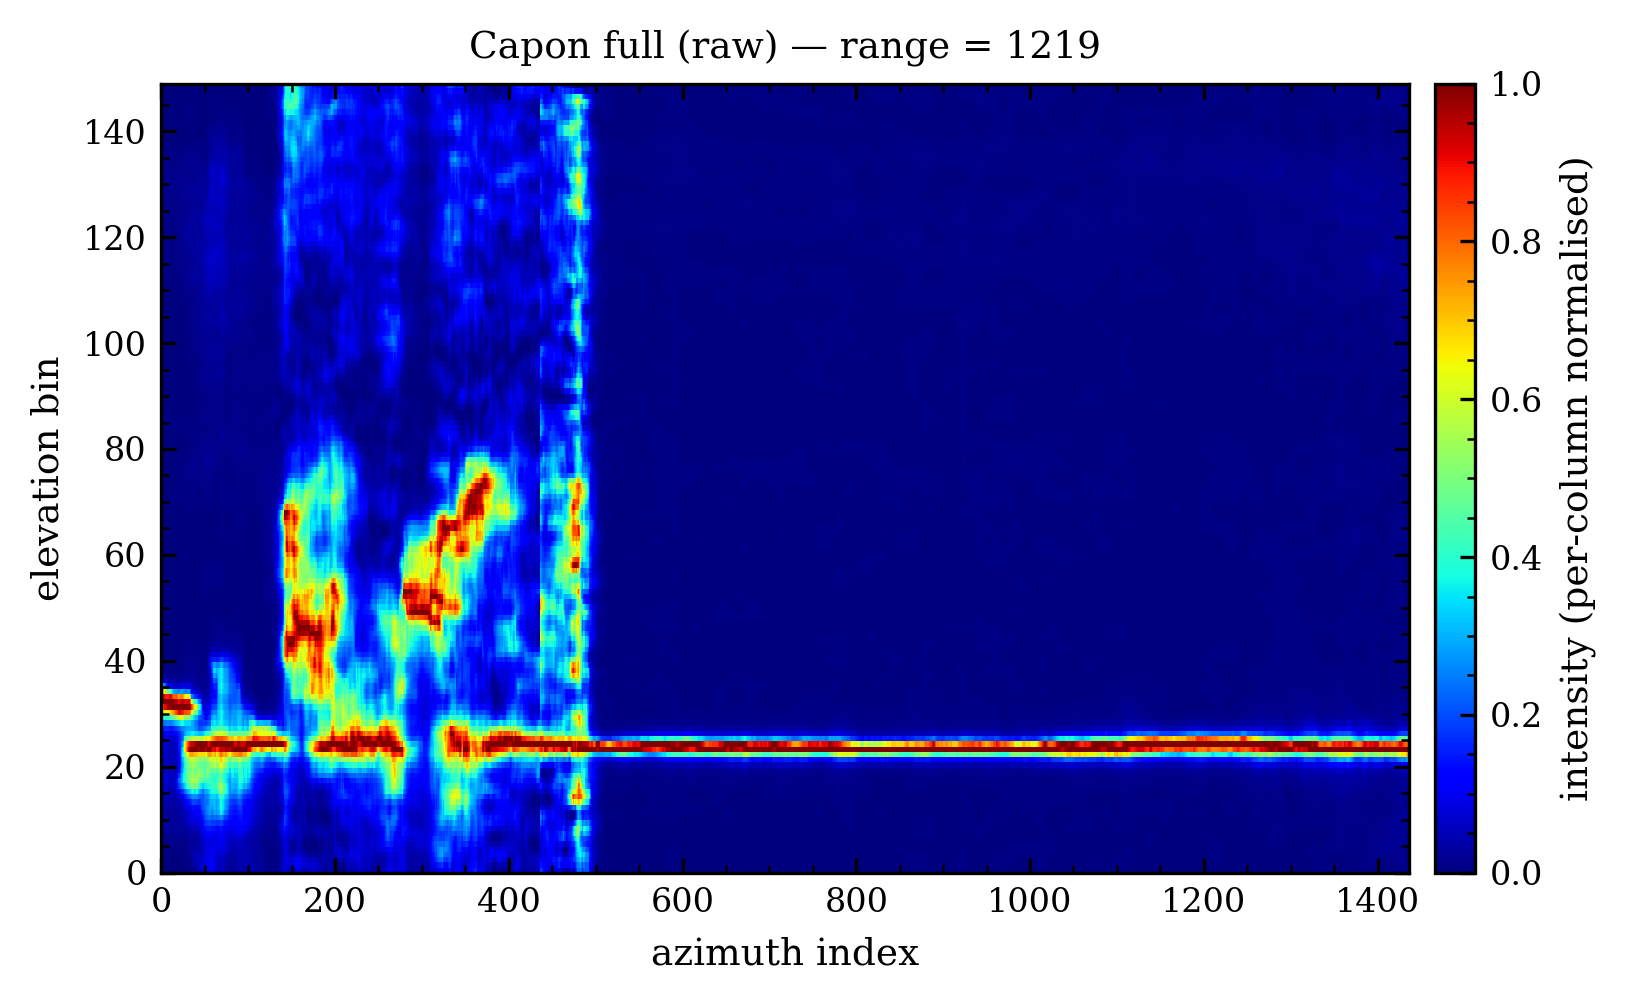
\includegraphics[width=\linewidth]{../figures/K2/dual_k2_ratio/cube_slices-90-10/cube_slices/az0331_rg1219/range_full_normalized.png}
    \end{minipage}\hspace{3pt}%
    \begin{minipage}[t]{0.345\textwidth}
      \centering
      {\small\textbf{\textcolor{good}{GT (Gaussian)}}}\\[3pt]
      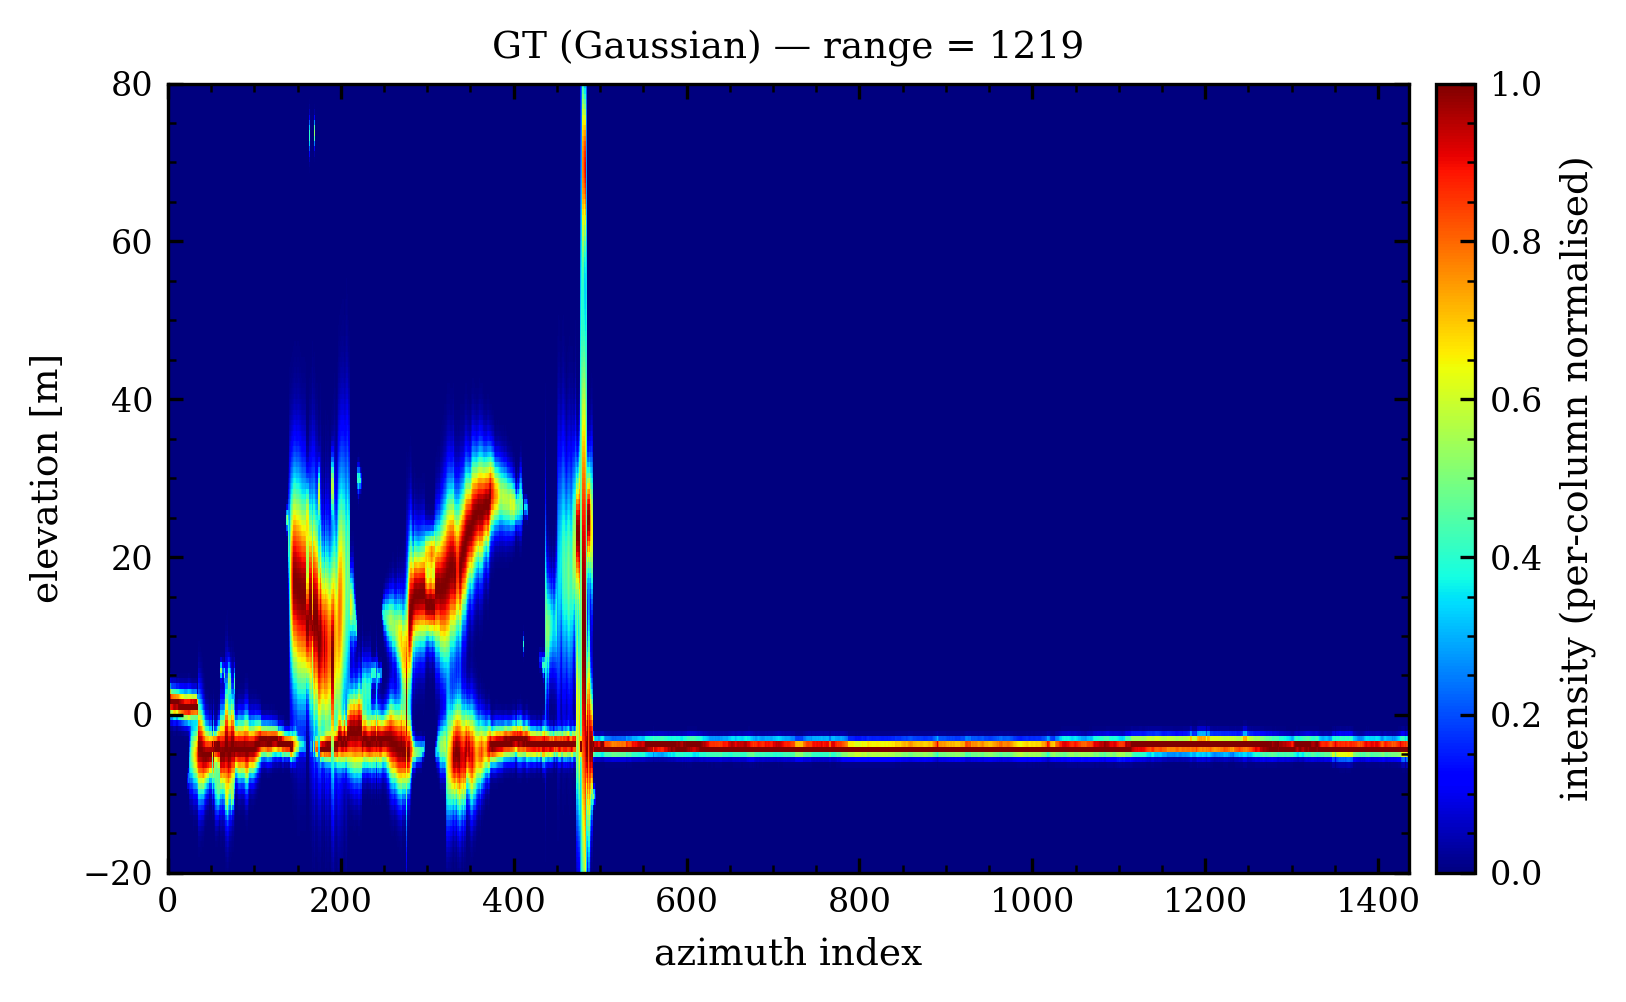
\includegraphics[width=\linewidth]{../figures/K2/dual_k2_ratio/cube_slices-90-10/cube_slices/az0331_rg1219/range_gt_normalized.png}
    \end{minipage}\hspace{3pt}%
    \begin{minipage}[t]{0.345\textwidth}
      \centering
      {\small\textbf{\textcolor{accent}{90--10 prediction}}}\\[3pt]
      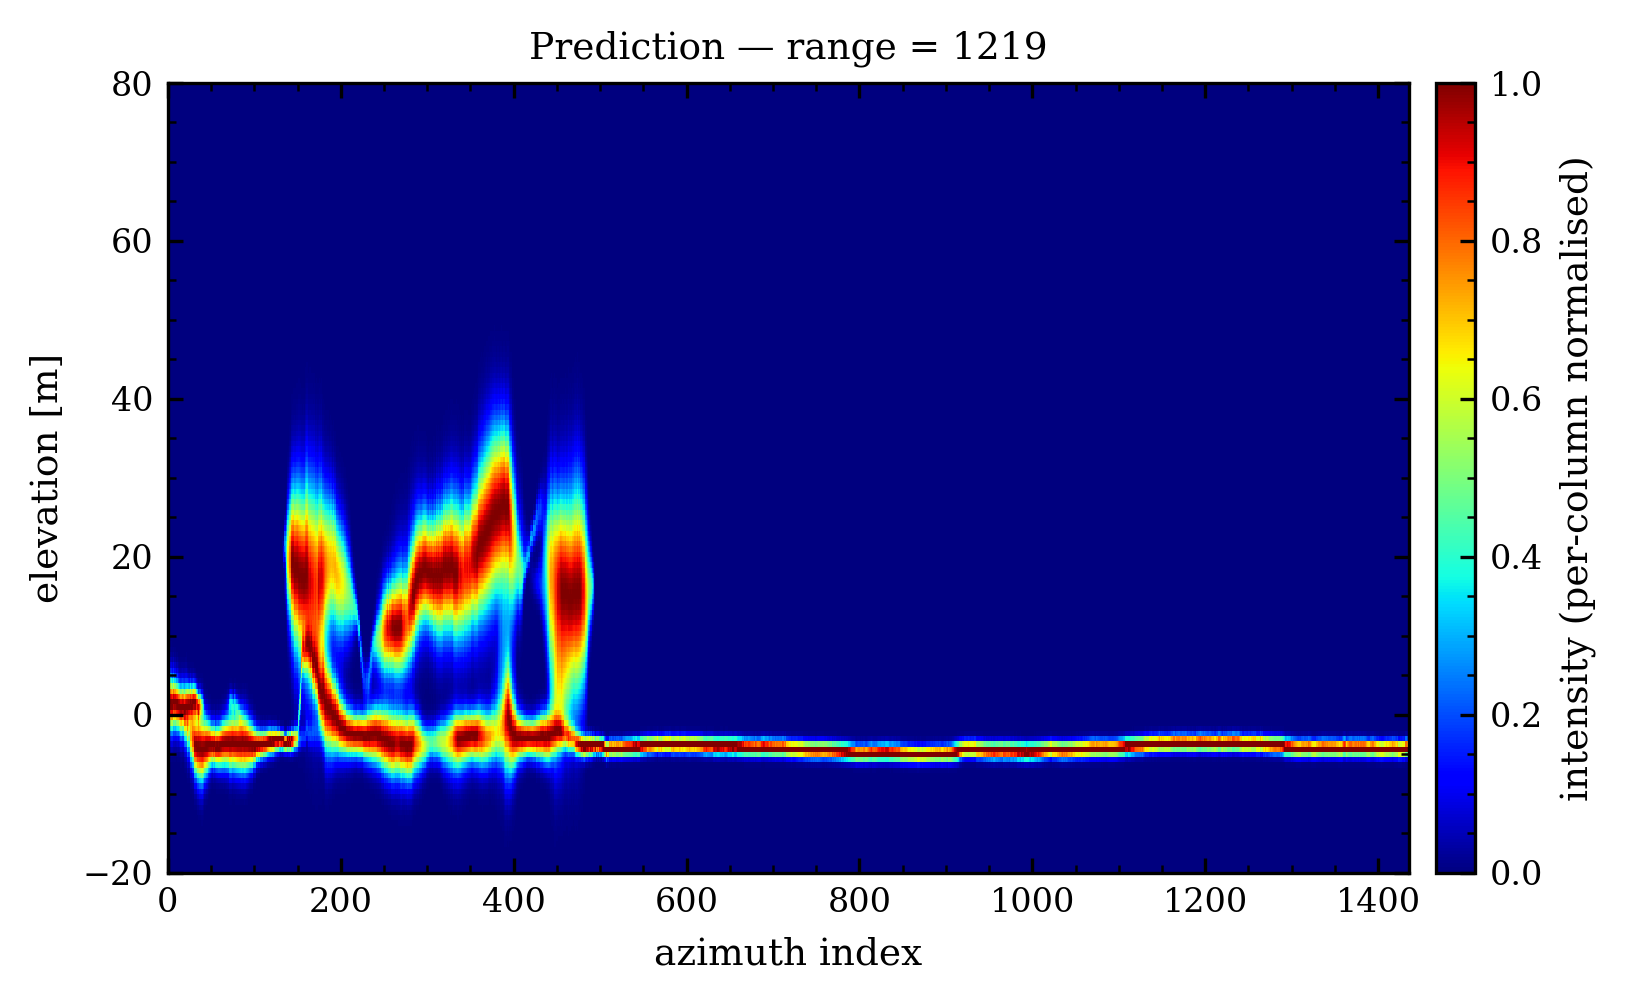
\includegraphics[width=\linewidth]{../figures/K2/dual_k2_ratio/cube_slices-90-10/cube_slices/az0331_rg1219/range_pred_normalized.png}
    \end{minipage}}
  \vspace{7pt}
  \parbox{0.90\textwidth}{\scriptsize\color{soft} Constant-range cut at $\mathrm{rg}=1219$, per-column normalised. The tomogram splits the scene before any fit: canopy clutter out to azimuth ${\approx}500$, then a single clean ground line to the swath edge. Label and prediction both follow that split, and the prediction holds the ground line at ${\approx}-4$\,m across the whole flat half. Its vegetated half comes out as broad smooth lobes where the label is filamentary --- the patch CNN regularises across neighbouring azimuths. The single-column GT streak at azimuth ${\approx}480$ sits on the tomogram's bright edge column but does not reach the prediction. Tomogram in elevation bins, the two mixture panels in metres.\par}
\end{frame}

% ---------------------------------------------------------------- 25x Ratio 90-10 slices: layered canopy
\begin{frame}{The 90--10 cube --- layered canopy over a continuous ground return}
  \centering
  \makebox[\textwidth][c]{%
    \begin{minipage}[t]{0.345\textwidth}
      \centering
      {\small\textbf{\textcolor{soft}{full-tomogram}}}\\[3pt]
      
\includegraphics[width=\linewidth]{../figures/K2/dual_k2_ratio/cube_slices-90-10/cube_slices/az1298_rg3230/range_full_normalized.png}
    \end{minipage}\hspace{3pt}%
    \begin{minipage}[t]{0.345\textwidth}
      \centering
      {\small\textbf{\textcolor{good}{GT (Gaussian)}}}\\[3pt]
      
\includegraphics[width=\linewidth]{../figures/K2/dual_k2_ratio/cube_slices-90-10/cube_slices/az1298_rg3230/range_gt_normalized.png}
    \end{minipage}\hspace{3pt}%
    \begin{minipage}[t]{0.345\textwidth}
      \centering
      {\small\textbf{\textcolor{accent}{90--10 prediction}}}\\[3pt]
      
\includegraphics[width=\linewidth]{../figures/K2/dual_k2_ratio/cube_slices-90-10/cube_slices/az1298_rg3230/range_pred_normalized.png}
    \end{minipage}}
  \vspace{7pt}
  \parbox{0.90\textwidth}{\scriptsize\color{soft} Constant-range cut at $\mathrm{rg}=3230$, per-column normalised. Two layers over roughly the first $850$ azimuths in all three panels: a ground return near $-6$\,m under vegetation at $15$--$25$\,m. The prediction keeps the separation, and the raised patch at azimuth $1130$--$1220$, where the return lifts to about $0$\,m before dropping back, shows in the tomogram, the label and the prediction alike. The thin GT column at azimuth ${\approx}790$ reaching past $60$\,m is cut short in the prediction --- isolated single-column towers are the failure mode these cuts keep showing. Tomogram in elevation bins, the two mixture panels in metres.\par}
\end{frame}

% ---------------------------------------------------------------- 25y Ratio 90-10 slices: dense canopy
\begin{frame}{The 90--10 cube --- dense canopy with a bare corridor}
  \centering
  \makebox[\textwidth][c]{%
    \begin{minipage}[t]{0.345\textwidth}
      \centering
      {\small\textbf{\textcolor{soft}{full-tomogram}}}\\[3pt]
      
\includegraphics[width=\linewidth]{../figures/K2/dual_k2_ratio/cube_slices-90-10/cube_slices/az1069_rg3466/range_full_normalized.png}
    \end{minipage}\hspace{3pt}%
    \begin{minipage}[t]{0.345\textwidth}
      \centering
      {\small\textbf{\textcolor{good}{GT (Gaussian)}}}\\[3pt]
      
\includegraphics[width=\linewidth]{../figures/K2/dual_k2_ratio/cube_slices-90-10/cube_slices/az1069_rg3466/range_gt_normalized.png}
    \end{minipage}\hspace{3pt}%
    \begin{minipage}[t]{0.345\textwidth}
      \centering
      {\small\textbf{\textcolor{accent}{90--10 prediction}}}\\[3pt]
      
\includegraphics[width=\linewidth]{../figures/K2/dual_k2_ratio/cube_slices-90-10/cube_slices/az1069_rg3466/range_pred_normalized.png}
    \end{minipage}}
  \vspace{7pt}
  \parbox{0.90\textwidth}{\scriptsize\color{soft} Constant-range cut at $\mathrm{rg}=3466$, per-column normalised: the densest of the four. Vegetation from azimuth $0$ to ${\approx}580$ and again from ${\approx}950$ out to the swath edge, with a bare corridor between them where only the ground return near $-7$\,m survives; the tomogram carries the same corridor. The prediction puts both blocks and the corridor in place and holds the sharp canopy wall at azimuth ${\approx}580$. Two costs: it picks the canopy back up at azimuth ${\approx}985$ against the label's ${\approx}955$, and the ${\approx}60$\,m point return near azimuth $1145$, visible in the tomogram as well as in the label, is missing. Tomogram in elevation bins, the two mixture panels in metres.\par}
\end{frame}
